% This LaTeX document needs to be compiled with XeLaTeX.
\documentclass[10pt]{article}
\usepackage[utf8]{inputenc}
\usepackage{ucharclasses}
\usepackage{amsmath}
\usepackage{amsfonts}
\usepackage{amssymb}
\usepackage[version=4]{mhchem}
\usepackage{stmaryrd}
\usepackage{caption}
\usepackage{graphicx}
\usepackage[export]{adjustbox}
\graphicspath{ {./images/} }
\usepackage{multirow}
\usepackage{underscore}
\usepackage[fallback]{xeCJK}
\usepackage{polyglossia}
\usepackage{fontspec}
\usepackage{newunicodechar}
\IfFontExistsTF{Noto Serif CJK TC}
{\setCJKmainfont{Noto Serif CJK TC}}
{\IfFontExistsTF{STSong}
  {\setCJKmainfont{STSong}}
  {\IfFontExistsTF{Droid Sans Fallback}
    {\setCJKmainfont{Droid Sans Fallback}}
    {\setCJKmainfont{SimSun}}
}}

\setmainlanguage{english}
\setotherlanguages{hungarian}
\IfFontExistsTF{CMU Serif}
{\newfontfamily\lgcfont{CMU Serif}}
{\IfFontExistsTF{DejaVu Sans}
  {\newfontfamily\lgcfont{DejaVu Sans}}
  {\newfontfamily\lgcfont{Georgia}}
}
\setDefaultTransitions{\lgcfont}{}

\title{LEVEL-INDEX ARITHMETIC : AN INTRODUCTORY SURVEY }

\author{F.W.J. Olver}
\date{}


\newunicodechar{→}{\ifmmode\rightarrow\else{$\rightarrow$}\fi}

\begin{document}
\maketitle
\captionsetup{singlelinecheck=false}


\section*{Foreword}
During the past few years, two teams have been pursuing research into the development and application of level-index arithmetic, one in Maryland, USA, and one in Lancaster, UK. The long-term members of the Maryland team are F.W.J. Olver and D.W. Lozier, their counterparts at Lancaster being C.W. Clenshaw and P.R. Turner: several others have made contributions, including S. Cramer, F. Golam-Hossen, R.E. Kaylor, I. Reid and C. Sims.

Each of the following seven lectures was prepared and presented by its named author, but it has been our intention that this set of seven should form a unified whole which will provide an introduction to the subject; we have collaborated in an endeavour to produce a compatibility of approach and to secure a uniformity of notation. The first two lectures prepare the way for their successors by demonstrating the motivation for seeking arithmetic systems other than floating point, and by describing some of the early responses to the need. The next four lectures describe the level-index system and its most important properties, show how it can be implemented and how it performs on some numerical examples. Finally, Lecture 7 points to the future by showing ways in which implementation may be made more efficient.

We should like to acknowledge the value of many helpful discussions, and particularly those with D.W.Lozier (National Bureau of Standards, Gaithersburg, Maryland), A. Feldstein (Arizona State University) and D. Parkinson (QMC, London).

We also acknowledge with gratitude the support we have received, through grants and contracts over several years, from the US Army Research Office, the National Science Foundation, the Science and Engineering Research Council and the Lancaster University Research Fund.

\section*{1: ALTERNATIVES TO FLOATING POINT - THE NEED }


\subsection*{1.1 Introduction}
In the first three lectures of this course, we shall be introducing various alternatives to the floating-point system of arithmetic and number representation within a computer. From Lecture 3 onwards the focus will be firmly on just one of these, the level-index system.

Before dealing with any particular proposed scheme, we should ask why we need to seek alternatives to the floating-point system. The primary purpose of this first lecture is to establish this need by considering the fascinating topic of the distribution of the leading significant digits of numbers and the implications of this for floating-point arithmetic.

After observing the well-used pages at the beginning of books of log. tables and then conducting an analysis of 20,229 numbers gathered from a varied host of sources, Benford [3] first suggested in 1937 that numbers are logarithmically distributed. Specifically, he conjectured that the frequency of leading significant digit (Isd), $n$, in radix $r$ is given by

$$
F^{(r)}(n)=\log _{r}(n+1)-\log _{r}(n) .
$$

This implies, for example, that $30 \%$ of decimally represented numbers have lsd 1 and that the frequency of 1sd $\mathbf{n}$ decreases steadily to about $\mathbf{4 . 6 \%}$ for 1sd 9 .

Since Benford's original work many authors have attempted to establish his conjecture. It is widely accepted as being fact by statisticians who allow for this distribution in the design of random number generators. Knuth [40] dedicates some nineteen pages to the phenomenon. Other justifications have been based on assumptions such as invariance to scaling or on the expected frequencies of Isd for the integers assuming some cut-off point. (See [20], [28], [53] and [54]). Hamming in [28] established that, once obtained, the logarithmic distribution is not disturbed by other arithmetic operations. He also showed that any reasonable distribution is moved closer, in a relative $L_{1}$ metric, to the logarithmic one by multiplication. The relevance of the logarithmic distribution to the study of errors in floating-point arithmetics has been studied, amongst others, by Barlow and Bareiss [2] and Goodman, Feldstein and Bustoz [22,23] and are discussed in Feldstein's lectures in this volume.

Section 1.2 will be concerned with establishing the validity of the logarithmic distribution in a way which seems more natural than the earlier approaches. Also in that section we\\
that the logarithmic distribution implies an immediate preference as to the choice of radix for floating-point arithmetic.

In Section 1.3 we go on to consider the consequences of the logarithmic distribution for the potential frequency of overflow and underflow in floating-point arithmetic. We see that in the absence of scaling of, or structure in, the problem being solved this risk can be alarmingly high. However any scaling or structure - which is typically inherent in physical problems - only replaces the overflow/underflow difficulty with a comparably worrying frequency of catastrophic cancellation causing serious loss of precision.

In Section 1.4 some conclusions are drawn and suggestions are made as to how a computer arithmetic should be designed to overcome these, apparently dual, hazards of the floating-point system.

\subsection*{1.2 The logarithmic distribution}
We begin this section with a justification of the logarithmic distribution based on the simple observation that the leading significant digit of a number is always potentially affected by multiplication or division whereas the lsd of a sum of two numbers is typically just that of the larger of the summands. It is therefore reasonable to consider the distribution of lsd resulting from repeated multiplication. We shall assume that the factors are taken from a uniform distribution. A full treatment of this can be found in [59].

For simplicity of description and notation we shall use the decimal base throughout and denote the frequencies of 1sd $n$ resulting from i multiplications by $F_{i}(n)$ for $n=1,2, \ldots, 9$ and $i=0,1,2, \ldots$. The corresponding continuous density functions will be denoted by $f_{i}$ so that


\begin{equation*}
F_{i}(n)=\int_{n}^{n+1} f_{i}(t) d t \tag{1.2.1}
\end{equation*}


It is not hard to obtain the following recurrence relation.


\begin{align*}
f_{i+1}(t) & =\frac{1}{9} \int_{1}^{10} \frac{1}{x} f_{i}(x) d x+\int_{t}^{10} \frac{1}{x} f_{i}(x) d x \\
& =\frac{10}{9} \int_{1}^{10} \frac{1}{x} f_{i}(x) d x-\int_{1}^{t} \frac{1}{x} f_{i}(x) d x \tag{1.2.2}
\end{align*}


\section*{THEOREM 1.2.1}
If $f_{i} \rightarrow f_{\infty}$ uniformly on $[1,10]$ as $i \rightarrow \infty$ then $f_{\infty}(t)=1 /(t \ln 10)$.

\section*{Proof}
If ( $f_{i}$ ) converges uniformly then the limit function satisfies the limit version of (1.2.2). It follows that $f_{\infty}$ is differentiable and satisfies the separable differential equation


\begin{equation*}
f_{\infty}^{\prime}(t)=-f_{\infty}(t) / t . \tag{1.2.4}
\end{equation*}


Hence $\mathrm{f}_{\infty}(\mathrm{t})=\mathrm{A} / \mathrm{t}$. Also

$$
\int_{1}^{10} f_{\infty}(t) d t=1
$$

from which it follows that $A=1 / \ln 10$.

From (1.2.2) we may deduce, by induction and integration by parts, that $f_{n}$ is a polynomial of degree $n$ in ( - In $t$ ). We can expand this polynomial using truncated exponential series for $1 / t=\exp (-\ln t)$. Thus we write


\begin{equation*}
f_{n}(t)=\sum_{i=0}^{n} c_{i}^{(n)} E_{i}(-\ln t) \tag{1.2.5}
\end{equation*}


where


\begin{equation*}
E_{i}(x)=1+x+\ldots+x^{i} / i! \tag{1.2.6}
\end{equation*}


Using (1.2.2) we find, for $0 \leqslant i \leqslant n$, that


\begin{equation*}
c_{i+1}^{(n+1)}=c_{i}^{(n)}=c_{n-i} \text {, say } \tag{1.2.7}
\end{equation*}


and


\begin{equation*}
c_{n+1}=\sum c_{n-i}\left[1-10 \mathrm{E}_{i+1}(-\ln t)\right] / 9 \tag{1.2.8}
\end{equation*}


Rearranging the series for $f_{n}$ in increasing powers of ( $-1 n t$ ) we deduce that ( $f_{n}$ ) is uniformly convergent provided that $\sum c_{i}$ is bounded and this in turn follows from the boundedness of the sequence $\left\{f_{n}(1)\right\}$. Full details of this argument can be found in [59]. Combining this result with Theorem 1.2.1 establishes

\section*{THEOREM 1.2.2}
The sequence $\left(f_{n}\right)$ converges to the limit $f_{\infty}$ and


\begin{equation*}
F_{\infty}(n)=\log _{10}(n+1)-\log _{10}(n) \tag{1.2.9}
\end{equation*}


In a subsequent paper [60] it was shown that none of the other arithmetic operations disturb this distribution. Thus, for example, multiplication of all numbers by a constant leaves the logarithmic distribution unchanged. One consequence is that the logarithmic distribution implies invariance to scaling, and so the earlier work establishing the logarithmic distribution under that assumption was simply half of a circular argument. It is also established in [60] that forming powers, taking roots or reciprocals (and, therefore, division) all leave the logarithmic distribution unchanged as do addition and subtraction. The observation that the arguments used to establish convergence above hold for any other (continuous) initial distribution implies that any number of other arithmetic operations could be included in the sequence of multiplications without affecting that convergence.

The combination of all these remarks amounts to a very strong justification of Benford's original conjecture that numbers are indeed logarithmically distributed. The frequencies of 1sd $n$ for the decimal system are given in the following table.

\begin{table}[h]
\begin{center}
\captionsetup{labelformat=empty}
\caption{Table 1.2.1 Frequencies (\%) of Isd for the decimal system.}
\begin{tabular}{lccccccccc}
n & 1 & 2 & 3 & 4 & 5 & 6 & 7 & 8 & 9 \\
$\mathrm{~F}_{\infty}(\mathrm{n})$ & 30.1 & 17.6 & 12.5 & 9.7 & 7.9 & 6.7 & 5.8 & 5.1 & 4.6 \\
\end{tabular}
\end{center}
\end{table}

Of course it follows from all the arguments presented above or elsewhere - and others! that $100 \%$ of binary represented numbers have leading significant digit 1 .

We conclude this section with a brief look at one immediate consequence of this distribution with respect to the choice of radix for floating-point representation. A more detailed description of these considerations can be found in [57]; we present here a simple comparison between the hexadecimal and binary representations.

A number X is represented in the (normalised) floating-point, base $\beta$, system by


\begin{equation*}
X= \pm f * \beta^{ \pm E} \tag{1.2.10}
\end{equation*}


where $\beta^{-1} \leqslant \mathrm{f}<1$ and E is an integer.

We shall compare the hexadecimal and binary systems using a hypothetical 32 -bit word with a positive representable range of $2^{-256} \leqslant \mathrm{X}<2^{256}$. At this stage we are not concerned with detailed electronic implementation of this representation and so may assume that the exponent range is balanced. (See also Feldstein's lectures in this volume).

Now $2^{256}=16^{64}$ and $64=2^{6}$ so that the hexadecimal word must allocate 6 bits to the exponent $E$ (and one for its sign). Allowing for the sign of the number $X$ this leaves 24 bits for the mantissa or fraction $f$. Similarly, since $256=2^{8}$, the binary word must have 8 bits (and a sign) allocated to the exponent. This leaves just 22 for the binary mantissa.

However since the leading significant digit of a floating-point binary number is 1 this need not be stored explicitly. Thus the binary format has an effective 23 bits for the mantissa.

Consider the representation errors associated with the storage of $X$ in these two forms. This can be gauged by the relative mesh sizes of the two systems, that is the gap between successive representations. Suppose the hexadecimal exponent of X is n , so that


\begin{equation*}
16^{n-1} \leqslant X<16^{n} \text { or } 2^{4 n-4} \leqslant X<2^{4 n} . \tag{1.2.11}
\end{equation*}


The difference between successive hexadecimal fractions is $16^{-6}$ (since the 24 mantissa bits represent 6 hexadecimal digits) and so the hexadecimal gap between X and its successor is $16^{\mathrm{n}-6}=2^{4 \mathrm{n}-24}$.

From (1.2.11), it follows that the binary exponent of X is $4 \mathrm{n}-3,4 \mathrm{n}-2,4 \mathrm{n}-1$ or 4 n and the difference between successive binary fractions is $2^{-23}$. Now the binary exponent is $4 n-3$ if and only if the leading significant hexadecimal digit, $\operatorname{lsd}_{16}(\mathrm{X})$, is 1 which occurs according to the logarithmic distribution with probability $1 / 4$. Similarly the binary exponent is $4 n-2$ if and only if $\operatorname{lsd}_{16}(\mathrm{X})=2$ or 3 and so on for the other cases. The following table summarizes the various possibilities. We see immediately that the probability that the binary representation having greater error than the hexadecimal one is only $1 / 4$ or, conversely the binary representation is more accurate than hexadecimal $50 \%$, and at least as good $75 \%$, of the time.

\begin{table}[h]
\begin{center}
\captionsetup{labelformat=empty}
\caption{Table 1.2.2 Comparison of hexadecimal and binary representation errors. $\mathrm{n}=$ hexademical exponent of X .}
\begin{tabular}{|l|l|l|l|l|}
\hline
$\operatorname{Isd}_{16}(\mathrm{X})$ & binary exponent & binary gap & hexadecimal gap & probability \\
\hline
1 & $4 \mathrm{n}-3$ & $2^{4 \mathrm{n}=26}$ & $2^{4 \mathrm{n}-24}$ & 1/4 \\
\hline
2,3 & $4 n-2$ & $2^{4 \mathrm{n}-25}$ & $2^{4 \mathrm{n}-24}$ & 1/4 \\
\hline
4,5,6,7 & $4 n-1$ & $2^{4 \mathrm{n}-24}$ & $2^{4 \mathrm{n}-24}$ & 1/4 \\
\hline
8,. . . , 15 & 4n & $2^{4 n-23}$ & $2^{4 \mathrm{n}-24}$ & 1/4 \\
\hline
\end{tabular}
\end{center}
\end{table}

There are several arguments based on probabilistic analyses of floating-point arithmetic which demonstrate advantages of the binary system relative to other bases. Some of these are presented at this meeting by Feldstein while others can be found in, for example, [21] and [23].

\subsection*{1.3 Overflow, underflow and cancellation}
In this section we consider two fundamental difficulties which can arise in floating-point computation and demonstrate that both can occur with disquieting frequency. We begin by considering the probabilities of overflow or underflow resulting from the add-magnitude and subtract-magnitude operations in a floating-point arithmetic system using the representation (1.2.10), that is

$$
X= \pm f * \beta^{ \pm E}
$$

We denote by $X^{+}$and $X$. the greatest and least representable positive numbers in the system. In a balanced system of floating-point arithmetic, we would have


\begin{equation*}
\mathrm{X}^{+} * \mathrm{X}_{-} \div 1 \tag{1.3.1}
\end{equation*}


Now the assumption of the logarithmic distribution implies that the fractions of floating-point numbers are logarithmically distributed and, assuming continuity of the distribution, that their exponents are uniformly distributed. Under this assumption it can be shown that the probability of overflow from add-magnitude is given by


\begin{equation*}
\mathbf{P}^{+}=\pi^{2} / 6\left(\ln \left(\mathbf{X}^{+} / \mathbf{X}_{-}\right)\right)^{2} \tag{1.3.2}
\end{equation*}


and the probability of underflow from subtract-magnitude is

$$
\mathrm{P}_{-} \neq \mathrm{P}^{+}
$$

(Detailed derivations can be found in [19]).

Define $E^{+}=\log _{2}\left(X^{+}\right)$and $E_{-}=\log _{2}\left(X_{-}\right)$. Then $E^{+}$and $E_{-}$are approximately the maximum and minimum binary exponents of representable numbers. For a balanced system $E_{-} \doteqdot-E^{+}$ and so it follows that


\begin{equation*}
\mathbf{p}^{+} \div \mathbf{K} /\left(\mathbf{E}^{+}\right)^{2} \tag{1.3.3}
\end{equation*}


where

$$
K=(\pi / \ln 2)^{2} / 24 \div 0.856
$$

Typically $E^{+}$is of the order of $2^{7}$ or $2^{8}$. Table 1.3.1, which is a shorter version of Table 2.4 of [19], demonstrates clearly the risk of overflow under this assumption of the uniform distribution of exponents for machines with various speeds and binary exponent ranges.

In practice, it would normally be the case for scientific computation that the problem is scaled by the choice of units. The effect is that the assumption of uniform distribution of exponents may well be invalid in such situations. Even in this case however the choice of units is made so that the input and final results are reasonably scaled rather than the intermediate results which could well have exponents near the extremes of the range. Sweeney's paper [58] presented a detailed statistical survey of major scientific computing programs. The assumption in Table 1.3.1 that just $5 \%$ of run-time is spent on add-magnitude operations is based on Sweeney's data.\\
(Addition time $=\mathrm{T} ; 1 \mu \mathrm{~s}=10^{-6}$ and $1 \mathrm{~ns}=10^{-9}$ seconds; assume $5 \%$ of run-time is used on add-magnitude).

One - minute run

\begin{table}[h]
\begin{center}
\captionsetup{labelformat=empty}
\caption{Table 1.3.1. Probability of overflow resulting from add-magnitude operations.}
\begin{tabular}{lccccc}
$\mathrm{T} \backslash \mathrm{E}^{+}$ & $2^{8}$ & $2^{12}$ & $2^{16}$ & $2^{20}$ & $2^{26}$ \\
$10 \mu \mathrm{~s}$ & 0.98 & 0.02 & 0.00 & 0.00 & 0.00 \\
100 ns & 1.00 & 0.78 & 0.01 & 0.00 & 0.00 \\
1 ns & 1.00 & 1.00 & 0.45 & 0.00 & 0.00 \\
\end{tabular}
\end{center}
\end{table}

One - hour run

\begin{table}[h]
\begin{center}
\captionsetup{labelformat=empty}
\caption{Table 1.3.1. Probability of overflow resulting from add-magnitude operations.}
\begin{tabular}{lccccc}
$\mathrm{T} \backslash \mathrm{E}^{+}$ & $2^{8}$ & $2^{12}$ & $2^{16}$ & $2^{20}$ & $2^{26}$ \\
$10 \mu \mathrm{~s}$ & 1.00 & 0.60 & 0.00 & 0.00 & 0.00 \\
100 ns & 1.00 & 1.00 & 0.30 & 0.00 & 0.00 \\
1 ns & 1.00 & 1.00 & 1.00 & 0.13 & 0.00 \\
\end{tabular}
\end{center}
\end{table}

One of the subjects Sweeney addressed was the distribution of exponent differences in addand subtract-magnitude operations. This topic was considered further by Feldstein and Goodman [17] who again concluded that the (hidden bit) binary system was the optimal floating-point arithmetic from the point of view of cancellation. We now address the problem of the frequency of catastrophic cancellation, that is where at least half of the significant digits are lost through cancellation in subtract-magnitude operations. The conclusions of [19] are summarised in Table 1.3.2 in which we consider the likelihood of losing 13 bits from a 27 -bit mantissa. (This is half the precision since the 27 -bit mantissa is equivalent to 26 bits together with the implicit or hidden leading bit).

\begin{table}[h]
\begin{center}
\captionsetup{labelformat=empty}
\caption{Table 1.3.2 Probability $P$ of catastrophic cancellation occuring at least once in $N$ subtract-magnitude operations.}
\begin{tabular}{ccccc}
N & 5 & 15 & 50 & 100 \\
P & 0.21 & 0.51 & 0.91 & 0.99 \\
\end{tabular}
\end{center}
\end{table}

We see that the frequency of such cancellation happening with fractions of length only 27 bits is very high. However the frequency of the loss of 13 bits would be unchanged for a much longer mantissa of say, 100 bits.

\subsection*{1.4 Conclusions and suggestions}
In the last section we saw that, under the assumption of the logarithmic distribution of 1sd, the risk of overflow can be alarmingly high - especially for the unwary programmer who performs no precautionary prescaling of the problem. This danger can be alleviated greatly by the use of a much greater exponent range using 26 bits " or 27 to account for the exponent sign or bias.

In the common situation where the problem is scaled either by the programmer or by the choice of units, the danger of catastrophic cancellation and a resulting loss of precision in the final output becomes a real worry. This can be countered by the use of a much greater mantissa length of perhaps 100 bits.

The combined effect of these possible safeguards would be a proposal for the use of a standard floating-point word for scientific computing of 128 bits consisting of the sign, the 100 -bit fraction and the biassed 27 -bit exponent. This proposal has substantial associated costs - both computational and financial. The storage requirement would be double to quadruple those for most current scientific computation. Arithmetic operations would inevitably be significantly slower than for conventional single or double length floating-point arithmetic and yet the benefits would probably be relevant only to large scale number-crunching.

The essential message is that in the floating-point environment improved machine speeds should be accompanied by the simultaneous increase of the exponent range and of the available relative precision. The alternative is to use some other arithmetic system in which the representable range is increased so as to reduce or eliminate the risk of overflow and underflow and in which the precision used is appropriate to the magnitude of the number.

The next lecture deals with several of the arithmetic systems which have been proposed with these ends in mind. One possibility is to retain the standard 32 or 64 bit word but with overflow/underflow from a reduced floating-point range into the level-index arithmetic first proposed by Clenshaw and Olver [8]. This possibility is discussed in [62]. The level-index system is the subject developed in the later lectures of this course.

It is worth commenting here that Benford in his original paper on the logarithmic distibution [3] suggested that nature does not count $0,1,2,3, \ldots$ but instead uses $0,1, e, e^{e}, \ldots$. These numbers, which we could term "Benford integers", are just the break points between different levels of the level-index system. In his 1985 address to the British Mathematical Colloquium [27], Hammersley argued that the Arabic number system itself was perhaps reaching its limits of usefulness in areas of physical and computation science and that some more compact notation was necessary for the representation of very large numbers. His most promising suggestion was for something similar to a base 2 level-index system.

From all the foregoing it is plain that alternatives to floating-point arithmetic are needed at least within special purpose and experimental scientific computing environments. The rest of the course is devoted to considering some of the possibilities, and level-index arithmetic in particular.

\section*{2: ALTERNATIVES TO FLOATING POINT - SOME CANDIDATES }


\subsection*{2.1 Introduction}
In the previous lecture we discussed some of the reasons for seeking alternatives to floating-point arithmetic for scientific computing. In particular, we highlighted the problems of overflow, underflow and cancellation. These considerations suggest the desirability of systems with a greater range of representable numbers and an appropriate precision for numbers of all magnitudes.

One major benefit of any new arithmetic which meets these requirements will be the saving in program development time and even perhaps run-time. These savings result from the removal of the need for programmers to scale problems so as to avoid difficulties such as overflow. Similarly, scientific software designers would no longer need to incorporate special code to handle exceptional situations which might result in overflow at an intermediate stage. Even if the arithmetic itself were to run more slowly, it may well be the case that these simpler programs would accomplish their tasks more quickly.

There are of course other reasons why alternative arithmetic systems may be wanted; these include special precision requirements in some particular range or some special purpose arithmetic for handling special data types. In this very brief survey of some of the recently suggested candidates, we shall concentrate largely on the number representations (and their ranges and precisions) of systems which are designed to overcome the problems of overflow and underflow. Time and space permit only an outline description of these systems and there are notable omissions. For instance there is no section on interval arithmetic; the review article [43] provides a full description and bibliography of this system. A good starting point for the interested reader on many of the systems would be the proceedings of the various IEEE Symposia on Computer Arithmetic, for example [38].

The next sections of this lecture contain brief descriptions of a number of systems which are typical of the differing approaches to computer arithmetic. In section 2.2 , we consider the CADAC system due to Hull and his coworkers ([32], [33] and [34]) which uses a decimal floating-point representation with dynamically variable range and precision and built-in exception-handling.

Section 2.3 is devoted to modified binary floating-point representations due to Matsui and Iri [45] and Hamada [25] both of which are designed to reduce the risks of overflow and underflow while retaining some of the familiarity of floating-point binary arithmetic. We\\
also consider a proposal of Kahan to utilise wrap-around characteristic with a counter to extend the range of conventional floating-point arithmetic.

In Section 2.4, we consider one of the rational arithmetics, namely the lexicographic continued fraction system of Kornerup and Matula [41] and [42]. One of the attractions of this system is the possibility of very rapid evaluation of complicated rational expressions in two variables.

Section 2.5 concludes this lecture with a brief comparison of the ranges and local precisions of some of these systems and the level-index and symmetric level-index systems [8], [9] and [10].

\subsection*{2.2 The CADAC system}
The CADAC (or Clean Arithmetic with Decimal base And Controlled precision) system has been developed over the past several years by Hull and his coworkers. It is much more than just an alternative computer arithmetic system since it has its own programming language which includes special facilities for exception handling and even user-defined exceptions for particular special situations. This last feature allows the possibility of automatic switching among different algorithms for the solution of a problem. For full details of the system see [32], [33] and [34].

CADAC uses decimal floating-point arithmetic with dynamically variable precision and range. The precision and range are related so that as the range is increased so is the number of significant digits - and vice versa. Specifically, a number is represented at precision $p$ as a normalised decimal floating-point number with $p$ digits in the mantissa, and exponent in the range $[-10 p, 10 p]$. The value of $p$ can be changed at any point in the program.

The programming language, Numerical Turing, is PASCAL-like and the precision of a variable is determined by the variable declaration. For example, the statement

\begin{verbatim}
var $\mathrm{a}, \mathrm{b}$ : real (10)
\end{verbatim}

declares the variables $a$ and $b$ to be 10 -digit normalised decimals with exponents in the interval $[-100,100]$ while

\begin{verbatim}
var a,b : real
\end{verbatim}

sets the precision of $a$ and $b$ to the current working precision; this is stored as the variable "currentprecision" which may be accessed and used within subsequent precision declarations.

The variability of the precision allows different parts of a routine to use different precisions so as to control the precision of the final result.

For example, the following routine has the effect of producing the inner product of two $n$-dimensional vectors with only one rounding error. This is effected by performing all the multiplications and accumulating the partial sums at the appropriate higher precision as explained below. This example is taken from [33].

Example 2.2.1 Computation of dot product in CADAC.

\begin{verbatim}
var dotproduct : real
begin
    precision:= currentprecision + getexp(n) +1
    var temp : real := 0.0
    for i := 1...n
        temp := temp + a(i)*b(i)
    endfor
    dotproduct := temp
end
\end{verbatim}

Note that the variable dotproduct is given the current working precision (of the calling program) on entry to the routine and that this precision is immediately increased by getexp(n)+1 for the internal working of the procedure. The function getexp obtains the (normalised decimal) floating-point exponent of its argument - which in this case is first converted to type real. The increased precision is exactly what is required to allow for all possible overflows, underflows or shifts within the accumulation of $n$ products of real numbers. The single rounding, at the precision level of $a, b$ and dotproduct, occurs in the abbreviation statement\\
dotproduct : $=$ temp.

We see that in some senses CADAC is not so much a new system of computer arithmetic as a familiar one being used together with dynamically controlled precision so as to reduce the risks of overflow, underflow and cancellation.

The other main feature of CADAC is its exception-handling. There are just three built-in exceptions - overflow, underflow and domainerror. The last of these is used for situations such as the square-root of a negative argument. However, the user has the freedom to define other exceptions and handlers to create, for example, automatic switches between different algorithms. Similarly, handlers can be attached to any routine so that appropriate action can be taken in the event of any of the built-in exceptions arising.

For example, it may be desirable in some applications simply to increase the precision - and therefore the range - in the event of overflow or underflow. There is not space to include details of these aspects here and the interested reader is referred to [32].

\subsection*{2.3 Overflow, underflow-free binary floating-point systems}
In this section we consider some of the suggestions that have been made for eliminating, or at least reducing, the incidence of overflow and underflow from binary floating-point arithmetic. Specifically we shall consider the representations of Matsui and Iri [45] and Hamada [25]. Before describing these in detail, however, we give brief consideration to a suggestion of Kahan made in a panel discussion at the IEEE Symposium on Computer Arithmetic in Como, May 1987.

The idea is simply to have a one-byte ( 8 bit) counter which represents as a binary integer the number of times a quantity has "wrapped around". When a result exceeds the floating-point range this counter is activated and, essentially, just registers the carries from the most significant end of the floating-point representation which itself wraps round so that the next representable number beyond $X^{+}$would be represented by 00000001 in the counter and a string consisting entirely of zeros in the original part of the word (allowing for the hidden bit). There seem to be several drawbacks to this. In terms of the storage requirement, it is necessary to know in advance which quantities are likely to overflow the standard range or to allocate this extra byte to every real variable. The latter course is equivalent to increasing the wordlength of the floating-point representation by eight bits all of which are allocated to the exponent. Such an increase in wordlength can, of course, be incorporated into any computer arithmetic system but it does not address the underlying problem.

If an extra eight bits were to be incorporated into, say, IEEE standard single-length floating-point format, it is also questionable as to whether they should all be allocated to increasing the exponent range. The use of 16 out of 40 bits for the sign and the biassed exponent seems excessive - especially in the light of the cancellation problem discussed in the previous lecture.

Even if it is known in advance which variables are likely to cause overflow or underflow, there are remaining difficulties: all internal routines must be able to support both data types, and the accumulators and temporary storage must all be designed for the 40 -bit word. For example, any one of the products or partial sums computed in the evaluation of a scalar product may overflow or underflow even though the final result is moderate in size. Effectively therefore all internal calculation would be in terms of the extended format as would all library function routines.

A suggestion that extra bits be incorporated into the representation of real numbers to increase range, precision or both can equally well be made for any system; it is not particularly relevant to the present discussion.

Matsui and Iri [45] advanced an extended floating-point format in which a variable portion of the computer word is allocated to storage of the exponent. Figure 2.3.1 shows the structure of the Matsui and Iri, "MI", 64-bit word.

\begin{figure}[h]
\begin{center}
\captionsetup{labelformat=empty}
\caption{Figure 2.3.1 Structure of a 64-bit MI word.}
  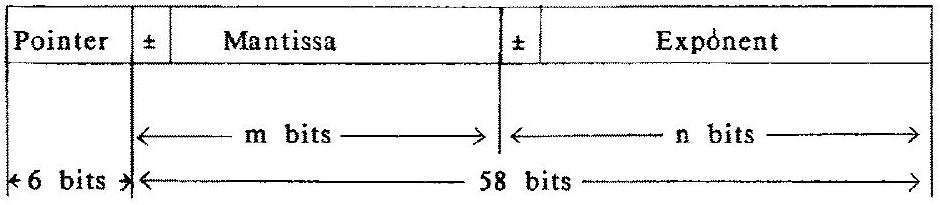
\includegraphics[alt={},max width=\textwidth]{cce78435-203d-4ce0-89c8-aaca04d3fe6b-16_205_940_629_254}
\end{center}
\end{figure}

The pointer registers the number of bits used for the signed exponent of a normalised binary floating-point representation.

For $|\mathrm{X}|$ close to unity, the exponent is small and is represented exactly with a small value of $n$. Consequently most of the 58 bits are available for the mantissa. As $|X|$ increases more bits are required for the (still exact) exponent and fewer are available for the mantissa. Thus the relative precision decreases as the magnitude of the number increases. Eventually the exponent occupies the full 58 bits and all relative precision is lost. At this point, Matsui and Iri's "level I" is used and the binary exponent of X is represented as a normalised floating-point number. That is, $X$ is represented as $\pm 2{ }^{f}{ }_{2}{ }^{E}$. Unless extra bits are allocated to the pointer to incorporate a "level indicator" very little of level 1 is available in the word described in Figure 2.3.1 which would only enable the pointer values 59, 60, 61, 62 and 63 to be used to determine how many bits are allocated to this exponent $E$ and the sign of $f$.

One question which arises immediately out of Figure 2.3.1 concerns the structure of the corresponding single-length MI format. Because the pointer would still require 5 bits, the single-length version would have only 27 for the two signs, the mantissa and the exponent. This renders the single-length format of MI insufficiently accurate for many purposes.

Although Matsui and Iri described MI arithmetic as overflow/underflow-free, this is not strictly true since the set of representable numbers is not closed under the basic arithmetic operations. For example, the product of two level-0 numbers could easily exceed the available range of the representation; however, with even a one-bit level indicator the range is, of course, increased greatly. Continuing this process leads effectively to a version of base 2 level-index arithmetic in which the index is represented in floating-point form.

The computational experience reported in [45] does not include any results which use representations beyond level 0 , and the arithmetic processes for handling such numbers are not described.

The final extended floating-point format to be considered here is Hamada's "Universal Representation of Real Numbers", or URR, [25,26]. This representation uses the same principle as MI arithmetic in that the mantissa and exponent are of variable length; but in URR the pointer is used as part of the exponent information. Specifically, we express a representable number X as


\begin{equation*}
\left.X= \pm f * 2^{ \pm\left(2^{m}\right.}+n\right) \tag{2.3.1}
\end{equation*}


where, after an initial sort,\\
m is stored as a unary integer,\\
n is a binary integer, m bits long and\\
$f \in[1,2)$ is the (hidden bit) binary mantissa.

The following example of the URR representation should help to clarify this.

Example 2.3.1 The URR representation of 57 is obtained as follows.

Step $1 \quad \mathrm{X}>0 \Rightarrow$ leading bit 0\\
$|X| \geqslant 1 \Rightarrow$ second bit opposite to first $\Rightarrow 01$\\
X $32 \Rightarrow$ third bit $1 \Rightarrow 011$

Step 2\\
For each i such that $\mathrm{X} \geqslant 2^{2^{\mathrm{i}}}(\mathrm{i}=1,2, \ldots)$ add another 1 and finally a 0 to mark the termination of this step.\\
Denote the number of 1's by m . In this case\\
$2^{2^{2}}=16 \leqslant \mathrm{X}<256=2^{2^{3}}$\\
so $m=2$ and representation is now 011110 .\\
Step 3\\
Find the $m$-bit integer $n$ such that

$$
2^{2^{m}+n} \leqslant X<2^{2^{m}+n+1}
$$

(Note that $n<2{ }^{m}$.)\\
For our example,

$$
2^{2^{2}+1}=32 \leqslant X<64=2^{2^{2}+2}
$$

so $\mathrm{n}=1$ and so we now have 01111001 .

Step 4 Find the mantissa in $[1,2)$ which is then represented using hidden bit binary.\\
For $\mathrm{X}=57$, we get the mantissa $1.1100100 \ldots 0$ and so the final representation is given by\\
$011110011100100 \ldots 0$\\
where we see that the 1 before the binary point of the mantissa is not stored explicitly.

The first three bits are the result of the initial sort, the next group (of three in this case) are the unary representation of $m(=2)$ followed by the 0 terminator. The third group is the binary integer representation of $n$ (this is $m$ bits long). The final group represents the mantissa in hidden bit binary form. (The spaces in the representation are here included only for clarity of demonstration).

Step 1 is an initial sort in which the sign and exponent sign of the representation are obtained. The number of consecutive l's after the leading three bits indicates the length of the exponent as well as forming part of it. For $\mathrm{X} \in(0,1), \mathrm{m}$ is represented as a string of 0 's followed by a 1 to mark its termination, while negative numbers are stored as the two's complement of their magnitude.

The above example and remarks also show how to interpret URR data which can then be processed by extensions of standard floating-point arithmetic - but with added complications, as follows.

Firstly, the exponent is not in simple binary form : this complicates the computation of shifts. Also, since mantissas are not necessarily of the same length their alignment and manipulation is even less straightforward. There is, as yet, no direct algorithm for URR arithmetic without separating data into two full words to represent the exponent and mantissa of the standard floating-point form.

Perhaps most importantly, URR does not eliminate overflow and underflow. However, the overflow level in Hamada's original description is precisely at the point at which all relative precision in the representation, is lost. This is seen by some advocates of floating-point arithmetic as being a significant advantage. This "advantage" only pertains because Hamada's choice was to cut the representation off at the point where the exact exponent could no longer be represented in the computer word. Thus if $2 n+3$ is greater than the number of bits available, then there is insufficient wordlength to represent $n$ exactly and the quantity overflows the URR system. Because of this, URR has many redundant representations which Hamada suggests should be used for NAN's (Not-A-Numbers) which, as with IEEE standard floating-point [37], can behave like infinity symbols or denote indeterminates. On the principle that some information is better than none, it seems to be to be more desirable to continue the URR representation by simply\\
carrying as much of the exponent as can be accommodated. The fact that such quantities would have no relative precision does not in itself render them worthless. (See Lectures 3 and 7, for example.) If necessary, the final few possible representations could still be reserved for the small number of NAN's needed by any system.

\subsection*{2.4 LCF arithmetic}
The LCF or lexicographic continued fraction system of computer arithmetic was developed by Kornerup and Matula [41]. This rational arithmetic grew out of their earlier work on fixed- and floating- slash arithmetic. Of course the fact that LCF is a rational arithmetic does not set it apart from the floating-point forms we have discussed hitherto; what is different is that it is overtly rational.

The representation is based on the fact that a nonnegative rational number $p / q$ can be uniquely expressed in the form


\begin{align*}
p / q=a_{0}+ & \frac{1}{a_{1}+\frac{1}{a_{2}+\frac{1}{a}}}  \tag{2.4.1}\\
& a_{m-1}+\frac{1}{a_{m}}
\end{align*}


where the integers $\left\{a_{i}\right\}$ satisfy $a_{0} \geqslant a_{i} \geqslant 1$ for $i \geqslant 1$ and $a_{m} \geqslant 2$ if $m \geqslant 1$. Denote this expression by $\left[\mathrm{a}_{0}, \mathrm{a}_{1}, \mathrm{a}_{2}, \ldots, \mathrm{a}_{\mathrm{m}}\right]$.

To enable compact representation of such a rational expression the lexicographic encoding of the integers is used. That is, the leading bit of the binary representation is replaced by the appropriate number of 1's followed by a 0 ; so that if the leading bit represents $2^{3}$, say, it is replaced by 1110 . The terminal 0 here acts as a separation between this leading "bit" and the rest of the binary representation whose length is determined by the number of 1's. For example, $27=16+8+2+1$ and so has the binary representation 11011. The lexicographic code replaces the leading 1 (which represents $2^{4}$ ) by 11110 and so 27 is stored as 111101011. The four leading 1's indicate that the remainder of the number occupies four more bits after the first 0 and so no further separator or indicator is needed to show that $\mathrm{a}_{\mathrm{i}}$ terminates here and that $\mathrm{a}_{\mathrm{i}+1}$ starts with the next bit.

Thus the representation (2.4.1) can be achieved by simply concatenating the lexicographic encoding of the integers $a_{0}, a_{1}, a_{2}, \ldots, a_{m}$. It is also the case that the natural ordering of the integers is preserved by this encoding and so discriminations between LCF numbers\\
are straightforward. The representation is readily extended to "signed" LCF to incorporate negative rationals, too. The LCF representation has no redundancy since there is a one-one correspondence between the irreducible fractions and the (theoretically infinite) set of LCF representations.

The arithmetic operations of the LCF system have been thoroughly researched by Kornerup and Matula who now have detailed hardware designs for LCF arithmetic chips. The operation of reciprocation is particularly simple since it only entails forming the 2's complement of the original quantity. The other arithmetic operations can be performed in a bit-serial manner so that, after a small start-up time, the result is produced bit-by-bit as the data is read bit-by-bit. Thus arithmetic can be performed in a time which is a linear function of the string length.

Recently in [42], Kornerup and Matula have extended this bit-serial algorithm so that rational expresssions of the form

$$
f(x, y)=\frac{a x y+b x+c y+d}{e x y+f x+g y+h}
$$

where $x$ and $y$ are in LCF form, can be evaluated in the same sort of way - again in linear time relative to the string lengths.

The LCF system can be used to provide a variable-precision, variable-range "real" computer arithmetic by allowing the string lengths to grow and using the ideas of "best rational approximation" to real numbers with the sequence of convergents $\left[a_{0}\right],\left[a_{0}, a_{1}\right]$, $\left[a_{0}, a_{1}, a_{2}\right], \ldots$. Such a sequence has quadratic oscillating convergence.

There is insufficient space to give more than the briefest of summaries of some of the important facts and results that Kornerup and Matula have obtained for this system - see [41], [42] for further details.

\subsection*{2.5 Summary and comparisons}
In the previous sections we have introduced various approaches to some of the problems of computer arithmetic which have included complete computing environments such as CADAC, modifications of the familiar floating-point systems and a completely different approach in the rational LCF arithmetic of Kornerup and Matula. In the first lecture we also mentioned the level-index system. The principal reason advanced for our study is the desire to overcome overflow and underflow while preserving a satisfactory measure of precision. In order to understand how well the various systems achieve these goals, we present in Table 2.5.1, a comparison of their overflow and underflow levels together with their mesh sizes at

1 and (approximately) $2^{255}$. These mesh sizes $\mu$ and $M$ are defined as the gaps between 1 and the next representable number, and between $2^{255}$ and its successor. LCF arithmetic is omitted from this table since its primary motivation is different from those of the other systems.

\begin{table}[h]
\begin{center}
\captionsetup{labelformat=empty}
\caption{Table 2.5.1}
\begin{tabular}{|l|l|l|l|l|l|l|l|l|}
\hline
\multirow[b]{3}{*}{CADAC} & \multicolumn{4}{|c|}{32-bit word} & \multicolumn{4}{|c|}{64-bit word} \\
\hline
 & X\_ & $\mathrm{X}^{+}$ & $\mu$ & M overflow & X。 & $\mathrm{X}^{+}$ & $\mu$ & M \\
\hline
 & $2^{-200}$ & $2^{203}$ & $2^{-20}$ &  & $2^{-431}$ & $2^{434}$ & $2^{-43}$ & $2^{207}$ \\
\hline
MI & $2^{-2^{25}-1}$ & $2^{2^{25}-1}$ & $2^{-25}$ & $2^{238}$ & $2^{-2^{56}-1}$ & $2^{2^{56}-1}$ & $2^{-56}$ & $2^{207}$ \\
\hline
URR & $2^{-2^{15}}$ & $2^{2^{15}}+1$ & $2^{-29}$ & $2^{240}$ & $2^{-2^{31}}$ & $2^{2^{31}+1}$ & $2^{-61}$ & $2^{208}$ \\
\hline
li & $2^{-28}$ & $\boldsymbol{>} \mathbf{2}^{\mathbf{2 5 5 3 6}}$ & $2^{-28}$ & $2^{237}$ & $2^{-60}$ & $\boldsymbol{>} \mathbf{2}^{\mathbf{6 5 5 3 6}}$ & $2^{-60}$ & $2^{206}$ \\
\hline
sli & $<2^{-2^{25536}}$ & $>2^{2^{\mathbf{2}}{ }^{\mathbf{6 5 5 3 6}}}$ & $2^{-27}$ & $2^{238}$ & $<2^{-2^{25539}}$ & $\boldsymbol{>} \mathbf{2}^{\mathbf{2}^{\mathbf{6 5 5 3 6}}}$ & $2^{-59}$ & $2^{207}$ \\
\hline
IEEE & $2^{-129}$ & $2^{127}$ & $2^{-23}$ & overflow & $2^{-1025}$ & $2^{1023}$ & $2^{-52}$ & $2^{207}$ \\
\hline
\end{tabular}
\end{center}
\end{table}

As in Lecture 1 the symbols X . and $\mathrm{X}^{+}$are used to represent the smallest and largest representable positive numbers. The values given here for $\mathrm{X}^{+}$for the IEEE floating-point system should actually all be multiplied by $\left(1-2^{-k}\right)$ where $2^{-k}$ is the precision of the mantissa. The values for the CADAC system are all approximate binary equivalents of the correct decimal quantities; the approximation is made for ease of comparison. (It is also the case that the word lengths chosen are not necessarily the most suitable for the decimal-based CADAC system).

Again, the $\ell i$ and sli figures are approximate values, but they demonstrate that although their mesh sizes do grow rapidly the relative precision at $2^{255}$ remains comparable with the systems of floating-point type. The Hamada (URR) and Matsui and Iri (MI) schemes also lose relative precision steadily as the magnitude increases but they, too, are comparable at this level. For the MI scheme the figures quoted for $\mathrm{X}_{\text {_ and }} \mathrm{X}^{+}$are for level 0 of their system for the reasons given in Section 2.3. For the URR system, likewise, the limits given are based on Hamada's suggestion that the exponent must be represented exactly.

\section*{3: LEVEL-INDEX ARITHMETIC }


\subsection*{3.1 Large numbers}
The aim of this lecture is to give a general and elementary introduction to level-index arithmetic. It is likely that questions will be raised more often than answered, but many of the answers should be forthcoming as the succeeding lectures unfold.

At the heart of this work, just as in some of the other work on new arithmetics which Peter Turner has outlined, is a concern with the two basic properties of the real numbers which we seek to represent and manipulate. These properties are magnitude and precision which, for computer arithmetic, have a crucial interdependence which has often been ignored in the past. In particular, floating-point arithmetic (flp), for all its attractive simplicity, has serious deficiencies in extreme (though not necessarily rare) situations, as has been shown here by both Alan Feldstein and Peter Turner.

On the one hand, any practical implementation of flp has a cut-off point. There is a largest representable number $\mathrm{X}^{+}$which can be easily exceeded by carrying out ordinary, simple arithmetic operations on numbers less than $\mathrm{X}^{+}$. On the other hand, the precision of flp numbers is always associated with relative error, even when this measure is utterly inappropriate. So ingrained has this measure become, that even experienced numerical analysts are inclined to assert that if a number has no correct significant figures then it is meaningless. It seems unfortunate that the expression "most significant figures" has been appropriated to describe the leading figures in the mantissa of a flp number, when it is clear that the information carried in the exponent is more important.

We shall return to this topic shortly; for the present we note the example given in [8]. Dirac estimated the ratio $M$, say, of the mass of the universe to the mass of a single proton to be about $10^{78}$, though the last digit of the decimal exponent is very uncertain. Clearly there are no correct significant figures in this estimate of $M$, and it would be meaningless to speak of its relative error. Nevertheless there is, equally clearly, important information in the estimate; we simply need a new error measure which will deal with very large numbers as readily as with those near unity. (We might indeed by tempted to refer to the relative error of the exponent in this example. In doing so, we should be setting off on the road to level-index arithmetic).

These, then, are the problems we address - a satisfactory treatment of magnitude and precision. It is our contention that level-index arithmetic ( $\ell$ i) provides just the framework we seek. First we define the li system.

Given any positive number $X$, we may represent it within the computer by its li-image $x$, which is obtained from $X$ by taking natural logarithms as many times as necessary (\& times, say) to bring the result ( $f$, say) into the interval $[0,1)$. For example, if $\mathrm{X}=1234567$ then $\ln \mathrm{X}=14.02623, \ln (\ln \mathrm{X})=2.640929$ and $\ln (\ln (\ln \mathrm{X}))=0.9711308$. The image x is then given by $\ell+\mathrm{f}$; in this example it is 3.9711308 . (Here $\mathrm{dX} / \mathrm{dx}=4.6 \times 10^{7}$, so if X is correct to the nearest integer then it is appropriate to record $x$ to seven decimal places). The numbers 2 and $f$ are the level and the index respectively, of the number $X$.

More concisely, we define the mapping function to be the generalized logarithm (gl) $\psi$, given by

$$
x=\psi(X)=1+\psi(\ln X)
$$

with $\mathrm{x}=\mathrm{X}$ for $0 \leqslant \mathrm{x}<1$.

The inverse function (whose existence is obvious) is the generalized exponential function (ge) $\phi$, given by

$$
X=\phi(x)=e^{\phi(x-1)}
$$

with $X=X$ for $0 \leqslant X<1$.

It may be noted that we could define other ge and gl functions (which would be equally suitable for 21 purposes) by changing the nature of $\psi$ and $\phi$ within $[0,1]$. In certain contexts this may be advantageous, as Lecture 7 will indicate; for the present, however, we use the functions defined above, by virtue of their formal simplicity.

It is easy to see that $\psi$ and $\phi$ are continuous, as are their first derivatives, but that there are discontinuities in their second derivatives at integer values of $x$.

The ability of $2 i$ arithmetic to deal with very large numbers is apparent from the above example; we may also note that the constant of Dirac to which we referred might be written as $M \div \phi(4.50)$, and we shall return to this example shortly when considering precision.

This ability cannot be achieved without paying some price, however. After all, in a fixed word-length of, say 32 bits, there are just $2^{32}$ different configurations of 0 's and 1 's. If some are to be used for representing very large numbers, then there will be fewer available for more moderate numbers. However, we argue, and we shall bring evidence to support our argument, that the redistribution of magnitude and precision brought about by li (as compared with flp ) is quite natural and wholly desirable.

\subsection*{3.2 Precision}
We now turn to the question of precision, and in this discussion we shall use the definitions given by Olver [48]. In his notation we have

$$
\bar{x} \propto x ; a p(\alpha, \quad \Leftrightarrow \quad \bar{x}=x+u ;|u| \leqslant \alpha,
$$

and

$$
\bar{x}=x ; r p(\alpha) \quad \Leftrightarrow \quad \bar{v}=x e^{v} ;|v| \leqslant \alpha .
$$

We say that $\bar{x}$ approximates $x$ with a precision (absolute in the first case, relative in the second) of $\alpha$. The former is conventional, while the latter differs from the conventional $\bar{x}=x(1+v)$ in second-order terms only. Olver's definition has the great advantage of symmetry ( $\bar{x} \approx x \Leftrightarrow x \approx \bar{x}$ ) and, because it is a metric, it is of ten more convenient in analysis.

When we are dealing with numbers of moderate magnitude (say unity or less) then the recording of numbers to fixed absolute precision is appropriate and convenient. (Consider, for example, familiar tables of elementary functions likes sines and cosines). With somewhat larger numbers we tend to use flp; that is to say we record to fixed relative precision. But when our numbers become very large then, as we have seen, this measure is inappropriate. However, with li arithmetic we have a ready-made alternative.

Let $X=\phi(x)$, where, for all nonnegative $X, x$ is recorded to a fixed absolute precision $\alpha$, say. Then, if $x<1$ (that is, $X$ is a level- 0 number), $X=x$ and is therefore itself given to absolute precision $\alpha$. If $1 \leqslant x<e$ then $X$ is a level-I number (in fact, $X=e^{X-1}$ ) and is given to relative precision $\alpha$. The generalisation beyond $x=e$ is obvious. We say that $X$ is given to generalized precision $\alpha$ when x is given to absolute precision $\alpha$ This uniform measure embraces the familiar measures for small and moderate numbers, and provides a logical extension for large numbers.

Returning briefly to Dirac's constant, we might say that $\mathrm{M}=\phi(4.50)$ to that number of figures. Conventionally, this implies that M is bounded below by $\phi(4.495) \div 2.93 \times 10^{75}$, and above by $\phi(4.505) \div 1.68 \times 10^{82}$. We do not know whether these bounds are in fact valid for this example: the point is that we are able to express any number, however large, in a concise and standard form that carries an indication of precision as well as of magnitude. Generally we shall write

$$
X=\phi(x) ; g p(\alpha) \quad \Leftrightarrow \quad X=\phi(\bar{x}) ;|\bar{x}-x| \leqslant \alpha
$$

\subsection*{3.3 Arithmetic operations}
The substantial theoretical advantages offered by $\ell$ i arithmetic lead us to consider the possibility of its implementation: that is, we examine methods for performing arithmetic\\
operations on numbers represented by their $\ell$ i images. To perform addition, for example, we shall need to be able to compute $z$, given $x$ and $y$, where

$$
\phi(z)=\phi(x)+\phi(y)
$$

This is a nontrivial task which we shall explore, but first we note that if we can devise acceptable methods for both addition and subtraction, then our task is complete. Other basic operations are essentially equivalent. For example, if

$$
\phi(z)=(\phi(x))^{\phi(y)}
$$

then, taking logarithms, we have

$$
\phi(z-1)=\phi(y) \phi(x-1)
$$

and again

$$
\phi(z-2)=\phi(y-1)+\phi(x-2)
$$

Thus powering, multiplication and addition are equivalent operations at different levels.

It is also relevant to note that the set of numbers for which we must construct addition and subtraction algorithms is limited by the fact that a very large $\ell i$ number is unchanged by the addition to it (or subtraction from it) of a smaller number, to any finite working precision. For example, to the implied precision,

$$
\phi(4.45678)+\phi(3.87654)=\phi(4.45678) .
$$

(Indeed, this result still holds with a gp of $10^{-9}$ ). We say that in this case, addition is trivial. This phenomenon is of fundamental importance, in theory and in practice, and it is treated in depth in Lecture 4. For now we quote just two pertinent results:

$$
\begin{aligned}
& \phi(5)+\phi(x)=\phi(5) ; g p\left(2^{-27}\right) \text { when } x \leqslant 5 \\
& \phi(6)+\phi(x)=\phi(6) ; g p\left(2^{-5,500,000}\right) \text { when } x \leqslant 6
\end{aligned}
$$

We may readily check that even to the moderate precision of 28 bp in the 8 image, some addition is nontrivial at level 5 , whereas even to $51 / 2$ million bp, all addition is trivial at level 6.

It is easy to conclude that, in implementing $\ell i$ arithmetic, it is both necessary and sufficient to allocate just 3 bits to the level.

\subsection*{3.4 Comparison of Ai with flp}
An early point to be made for the flp system is that it represents small numbers as readily, and as accurately, as large numbers. We see that $\ell$ i may be given a similar property by allocating a single special bit to denote reciprocation; we express any number less than unity in the form $X=(\phi(x))^{-1}$. This bit plays a role similar to that of the sign of the exponent in flp . Where it is desirable to distinguish this modified $\ell \mathrm{i}$ system from the original scheme, we shall call it the symmetric level-index (sti) system.

An alternative notation for sli introduces a new mapping function $\Psi$ defined by

$$
\Psi(X)=\left\{\begin{array}{l}
\psi(\ln X) \text { for } X \geqslant 1 \\
-\psi(-\ln X) \text { for } X<1
\end{array}\right.
$$

The corresponding inverse function is $\Phi$, where

$$
\Phi(x)= \begin{cases}e^{\phi(x)} & \text { for } x \geqslant 0 \\ e^{-\phi(-x)} & \text { for } x<0\end{cases}
$$

To make a specific comparison with flp , we now suppose that we have a computer word of 32 bits, and we weigh orthodox flp against sli. The flp system will need two of its bits for signs, and will typically allocate 7 to the exponent, leaving 23 for the mantissa - which effectively becomes 24 when we take the "hidden" bit into account. The largest representable number is $2^{127}\left(1-2^{-24}\right)$.

The sli system will also need the two sign bits (one of these being the reciprocation bit mentioned above) and, as we have seen, 3 are needed for the level. Thus 27 are available for the index. The largest representable number is $\$\left(8-2^{-27}\right)$, which is much too large to be written in flp form. (If high precision is not needed in our very small numbers, then we can use 2 i , as opposed to sli, and 28 bits are available for the index).

It is not difficult to show that the precision offered by the two systems is similar for numbers around 1000 ; sli is rather better for smaller numbers, flp for larger numbers until, of course, they become as large as $2^{127}$. At that point flp fails abruptly, while sli continues to operate, and to provide the uniform precision $\mathrm{gp}\left(2^{-27}\right)$.

An argument might be raised to the effect that the abolition of overflow is not to be desired: certainly some writers of scientific programs tend to regard the appearance of overflow in flp computations as a useful indicator of error, either in the coding or in the underlying numerical analysis. Such diagnostic considerations have an undeniable validity,\\
but it should be noted that $\ell i$ arithmetic permits their more logical resolution. Whenever any computed quantity exceeds some bound B , say, then this fact may be brought to the user's attention. This number $B$ could reasonably be given the default value $\phi(6)$ perhaps, and of course the user would have the option of changing it. He would be able to abort the calculation when $B$ was exceeded if he so wished; otherwise the program would continue. The user could also, in any case, be given an indication of the largest number (in modulus) generated by his program. This situation seems preferable to the familiar one in which a bound is set arbitrarily by the system for all programs, most of which will fail completely when it is exceeded. (Also see [16]).

A deeper comparison will be described in Lecture 4 and further details may be found in [44]:

\subsection*{3.5 Addition and subtraction}
Later lectures will treat details of implementation, and possibilities for the future. We now deal with the fundamental algorithms for addition and subtraction in broad outline, first in ordinary li (not sli) arithmetic.\\
We take the basic problem to be the computation of $z$ from $x$ and $y$, where


\begin{equation*}
\phi(\mathrm{z})=\phi(\mathrm{x}) \pm \phi(\mathrm{y}) ; \mathrm{x} \geqslant \mathrm{y}>0 . \tag{3.5.1}
\end{equation*}


We shall use $\ell, m$, and $n$ to denote the levels of $X=\phi(x), Y=\phi(y)$, and $Z=\phi(z)$ respectively, while $f, g$, and $h$ denote the corresponding indices. Then we define sequences

$$
\begin{array}{ll}
a_{j}=1 / \phi(x-j), & j=\ell-1, \ell-2, \ldots, 0, \\
b_{j}=\phi(y-j) / \phi(x-j), & j=m-1, m-2, \ldots, 0, \\
c_{j}=\phi(z-j) / \phi(x-j), & j=0,1, \ldots .
\end{array}
$$

The sequences $\left\{\mathrm{a}_{\mathrm{j}}\right\}$ and $\left\{\mathrm{b}_{\mathrm{j}}\right\}$ are computed to a fixed absolute precision. Efficient routines are needed for this purpose; they may be built upon the relations

\[
\begin{array}{ll}
a_{j-1}=e^{-1 / a_{j}}, & a_{\ell-1}=e^{-f} \\
b_{j-1}=e^{-\left(1-b_{j}\right) / a_{j}}, & b_{m-1}=a_{m-1} e^{g} . \tag{3.5.6}
\end{array}
\]

Then we may compute the value of $c_{o}$ from the equation


\begin{equation*}
c_{o}=1 \pm b_{o} \tag{3.5.7}
\end{equation*}


which is an immediate consequence of (3.5.1) on division by $\phi(x)$. The remainder of the sequence $\left(c_{j}\right)$ may then be calculated, from


\begin{equation*}
c_{j}=1+a_{j} \ln c_{j-1}, \tag{3.5.8}
\end{equation*}


(We note that the "c-relation" (3.5.8) is the same as the "b-relation" (3.5.6) except that it proceeds in the opposite direction). The c-relation is continued until there is a value such that $\mathrm{c}_{\mathrm{j}}<\mathrm{a}_{\mathrm{j}}$. Then

$$
z=n+h, \quad \text { where } n=j, \quad h=c_{j} / a_{j}
$$

Several special cases need to be treated, and several important points need further investigation; not least the question of the precision to be carried in the various quantities. Full details can, however, be found in [9]. This reference includes a detailed error analysis of the algorithm, and shows that by carrying a specific number of extra bits in the sequences we can ensure that the accumulation of round-off error is small compared with the unavoidable errors caused by roundings in the $x$ and $y$. (Indeed, we can make the error arbitrarily small.)

The implementation of $s l i$ requires a few simple variations; we find that in detail some of these are simplifications rather than complications.\\
We must consider operations like

$$
\begin{aligned}
& \phi(z)=\phi(x)+\phi(y) \\
& \phi(z)=\phi(x)+1 / \phi(y) \\
& 1 / \phi(z)=1 / \phi(x)+1 / \phi(y)
\end{aligned}
$$

In each case we suppose that the first term on the right is the larger. For simplicity, we now refer to these three cases as "large", "mixed" and "small" arithmetic respectively. The approach is as before, but the sequences generated vary. The large case is the one already treated by $\ell i$, of course, and we need not refer to it again.

In the mixed case we use the same $\left(\mathrm{a}_{\mathrm{j}}\right)$ and $\left(\mathrm{c}_{\mathrm{j}}\right)$ sequences as before, but instead of the b -sequence we compute

$$
\alpha_{\mathrm{j}}=1 / \phi(\mathrm{y}-\mathrm{j}),
$$

and in this case the linking equation is

$$
c_{0}=1+a_{0} \alpha_{0}
$$

For small arithmetic we again compute the $\left\{\mathrm{a}_{\mathrm{j}}\right\}$ and $\left(\mathrm{c}_{\mathrm{j}}\right)$ as before, but now the $\left\{\mathrm{b}_{\mathrm{j}}\right\}$ are replaced by

$$
B_{j}=\phi(x-j) / \phi(y-j),
$$

and the linking equation by

$$
1 / c_{0}=1+\beta_{0} .
$$

Reference [10] contains a detailed analysis of the fundamental sli algorithm. The purpose of the present brief account is to indicate that it is possible to carry out $\ell i$ and sli arithmetic by using algorithms which generate numbers of moderate magnitude in fixed precision. Further research will be aimed at producing faster algorithms.

\section*{4: CLOSURE AND PRECISION }


\subsection*{4.1 Closu e}
In preceding lectures we have heard how the $\ell i$ and $s \ell i$ systems were introduced to combat the problems of overflow and underflow, and seen how arithmetic operations can be carried out in these systems. We have also seen that with quite modest values of the 2 i image x it is possible to represent numbers $X=\phi(x)$ that lie far beyond the ranges of representable numbers of all other existing and proposed systems, including those of Matsui and Iri [45] and Hamada [25]. Nevertheless, it might be argued that even with the $\ell i$ systems overflow is still possible. This is indeed so. However, overflow is impossible within the framework of arithmetic operations (other than division by zero) in finite-precision arithmetic. We begin with an explanation of this statement.

To fix ideas, let us suppose that the internal arithmetic base of the computer is $r$, and the fractional parts of the $\ell i$ images are stored to $d$-nary places. Then if we add any positive representable number $\phi(x)$ to itself the stored $\ell$ i image of the sum will not exceed $x$, provided that


\begin{equation*}
\phi\left(x+c r^{-d}\right)>2 \phi(x) . \tag{4.1.1}
\end{equation*}


Here $c$ is a positive constant: if the $\ell$ arithmetic processor computed to infinite precision, then we would have $\mathrm{c}=1$ for chopping, and $\mathrm{c}=1 / 2$ for rounding. By using a sufficient number of guard digits in the processor we can approach these values arbitrarily closely, but the precise value of $c$ is unimportant. On taking logarithms the inequality (4.1.1) becomes

$$
\phi\left(x-1+c r^{-d}\right)>\phi(x-1)+\ln 2 .
$$

If $x>2$, then $\phi^{\prime}(x-1)$ is increasing. Hence by application of the mean-value theorem we see that the last inequality is satisfied when

$$
\operatorname{cr}^{-\mathrm{d}} \phi^{\prime}(\mathrm{x}-1) \geqslant \ln 2
$$

This is equivalent to

$$
x \geqslant x\left(c^{-1} r^{d} \ln 2\right)+1
$$

where $x=\chi(t)$ is the inverse function to $t=\phi^{\prime}(x)$.

Sample values of $\chi(t)$, computed with the aid of Newton's rule, are as follows:

$$
\chi\left(2^{32}\right)=4.06 \ldots, \quad \chi\left(2^{64}\right)=4.26 \ldots, \quad \chi\left(2^{5,502,869}\right)=5.00 \ldots
$$

Consider now the set $A$ of all numbers generated by the addition or subtraction of any two numbers, beginning with any pair of numbers whose $\ell i$ images are numerically less than $\chi\left(e^{-1} r^{d} \ell n 2\right)+1$. Assume that the $\ell i$ images of the members of $A$ are generated by arithmetic operations in the 2 i system and stored to d r-nary places. In consequence of the result just established, the absolute values of the members of $A$ are bounded by $\phi\left(X\left(c^{-1} r^{d} \ell n 2\right)+1\right\}$. In a sense $\phi\left\{X\left(c^{-1} r^{d} \ell n 2\right)+1\right\}$ represents "infinity", or rather, an "upper bound for infinity", for the operations of addition and subtraction. If we extend the arithmetic processes to include multiplication and division, other than division by zero, then the set of numbers so obtained is bounded in absolute value by $\phi\left(\chi\left(e^{-1} r^{d} \ln 2\right)+2\right)$. This is a consequence of the equivalence of multiplication and division to addition and subtraction at one level below; for example,

$$
\phi(z)=\phi(x) \phi(y) \quad \Leftrightarrow \quad \Leftrightarrow(z-1)=\phi(x-1)+\phi(y-1),
$$

when $x, y \geqslant 1$.

We have therefore, shown that when the $\ell i$ system is used with any finite-precision arithmetic, there is a subset of its set of representable numbers that is closed under the operations of addition, subtraction, multiplication and division, excluding division by zero. Obviously, the same conclusion also applies to the sti system.

From the numerical values of $\chi(t)$ quoted above, it follows that with $r=2$ and $d=32$, that is, with 32 bits assigned to the storage of the fractional part of the $\ell i$ image, an upper bound for the absolute values of numbers generated by addition and subtraction is $\phi(5.07)$, whether the abbreviation mode be chopping or rounding. For multiplication and division the corresponding bound is $\$(6.07)$. To raise the overall upper bound from $\phi(6.07)$ to $\phi(7)$, or higher, we would need a wordlength in excess of $5,500,000$ bits. Thus, in practice, levels beyond 6 will not be entered; in consequence it will always suffice to allocate 3 bits to the storage of the integer part of the ti image.

Once again, it could be argued that the closure property is not peculiar to the $\ell i$ and the sti systems. When the floating-point system is augmented by the additon of NAN's ("Not-A-Numbers") [37] it can be regarded as being closed. However, NAN's are artificial and their occurrence signals a complete loss in precision. In contrast, the approach to infinity in the $\ell i$ and the $s \ell i$ systems is completely natural, and the appropriate measure of precision (gp) is maintained.

\subsection*{4.2 Precision}
For the fixed-point system the appropriate error measure is absolute error. For the floating-point system the appropriate error measure is relative error, or more satisfactorily, relative precision. For the $\ell i$ and the sli systems the appropriate error measure is generalized precision, that is, the absolute error in the 2 i or sli image. (See Lecture 3.)

How can we compare, say, relative precision and generalized precision? Suppose that $\mathrm{X} \geqslant 1$ and the $\ell i$ image $x$ of $X$ is correct to $d$ places in base $r$. (By "correct" we mean correctly chopped or correctly rounded.) The maximum relative error in $X$ is $\left\{\varphi^{\prime}(x) / \phi(x)\right\} r^{-d}$ Therefore a measure $m$, say, of the number of correct digits in the mantissa of the corresponding floating-point form of X is given by

$$
m=d-\log _{r}\left\{\phi^{\prime}(x) / \phi(x)\right\}
$$

Since

$$
\phi^{\prime}(x) / \phi(x)=\phi^{\prime}(x-1)=\phi(x-1) \phi(x-2) \ldots \phi(x-2+1),
$$

where $1(31)$ is the integer part of $x$, we have


\begin{equation*}
m \div d-\log _{r} e \cdot \phi(x-2) \tag{4.2.1}
\end{equation*}


Now let $\lambda$ and $\mu$ denote the exponent and mantissa, respectively, of the normalized floating-point form of X ; thus

$$
\phi(x)=r^{\lambda} \mu, \text { with } 1 / r \leqslant \mu<1 .
$$

Then the number of digits, $n$ say, in $\lambda$ is represented by $\log _{r} \lambda$. On taking logarithms we have

$$
\phi(x-1)=\lambda \ln r+\ln \mu
$$

and, as long as $x \geqslant 2$,

$$
\phi(x-2)=\ln \lambda+\ln \ln r+\ln \left[1+\frac{\ln \mu}{\lambda \ln r}\right] \div \ln \lambda
$$

Hence


\begin{equation*}
\log _{r} e \cdot \phi(x-2) \div \log _{r} \lambda=n \tag{4.2.2}
\end{equation*}


Combination of (4.2.1) and (4.2.2) yields

$$
n+m \neq d
$$

In words, in the corresponding floating-point form of X , the number of digits in the exponent plus the number of correct digits in the mantissa approximately equals the number of correct places in the ti image of X .

The result just derived provides a rough, but useful, practical guide. However, for very large values of $X$ it breaks down. More accurate information can be arrived at as follows.

Suppose, for example, that $r$, the internal arithmetic base, is 2 and the computer word has 32 bits. According to the IEEE standard [37] one of these bits is allocated to the sign of the represented number $X$, one is allocated to the sign (or bias) of the exponent, and 7 are allocated to the exponent itself. This leaves 24 for the mantissa (after allowing for the hidden bit). This arrangement is indicated schematically by the trapezium OABC in Figure 4.2.1. In this diagram, the vertical scale is $\xi \equiv \log _{2} \log _{2} X$. Since $\xi \geqslant 0$ this means we are considering values of $X$ such that $X \geqslant 2$. The triangular part to the left of the $\xi$-axis represents the digits actually used for this exponent, whereas the rectangular part to the right of the $\xi$-axis represents the digits assigned to the mantissa. Overflow takes place at the horizontal boundary BC .

\begin{figure}[h]
\begin{center}
  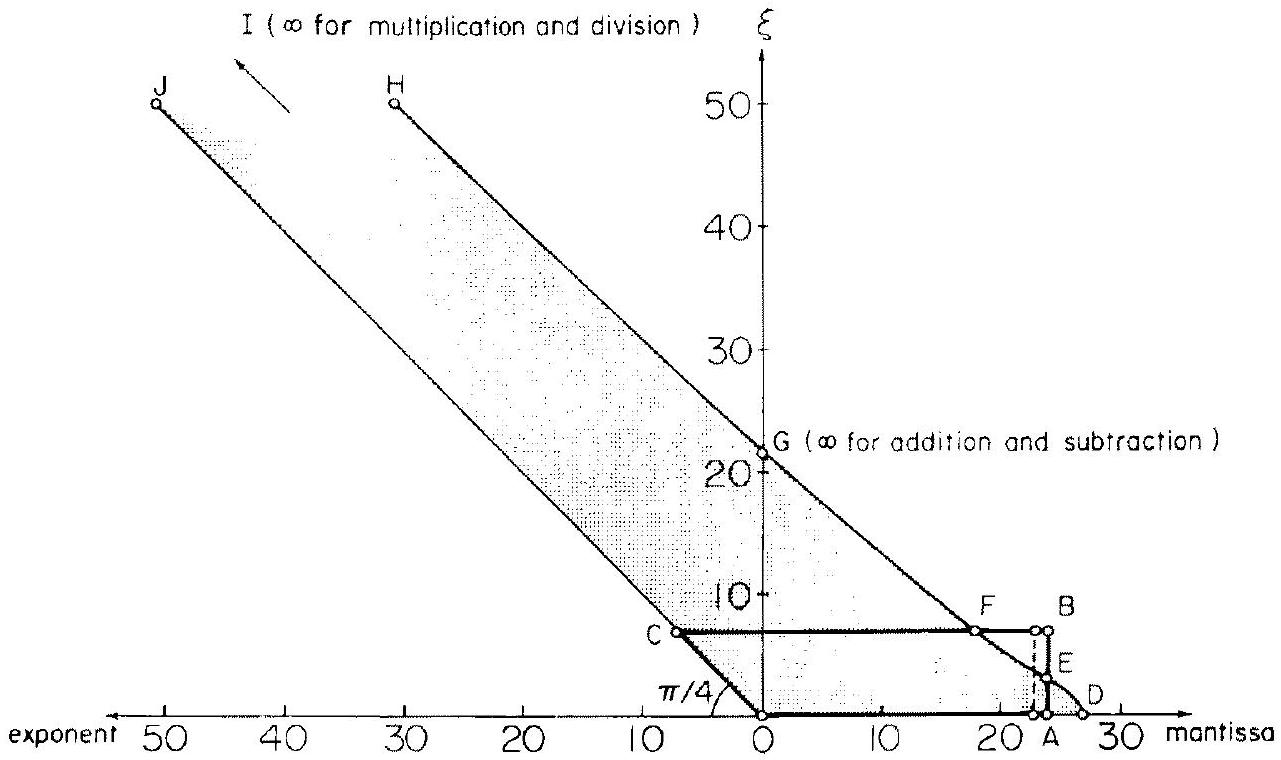
\includegraphics[alt={},max width=\textwidth]{cce78435-203d-4ce0-89c8-aaca04d3fe6b-33_760_1281_1159_187}
\captionsetup{labelformat=empty}
\caption{Figure 4.2.1. Accurate bits, in floating-point form, of the IEEE standard word and the corresponding sti word. (Approximately to scale).}
\end{center}
\end{figure}

With a 32-bit word in the sli system we allocate one bit to the sign of $X$ and 4 bits to the integer part and sign (or bias) of the sli image $x$. This leaves 27 bits for the fractional part of $x$. The absolute change $\delta X$, say, in $X$ resulting from an increase of 1 unit in the last place of $x$ is therefore given by

$$
6 \mathrm{X}=\Phi\left(\mathrm{x}+2^{-27}\right)-\Phi(\mathrm{x})=\Phi\left(\mathrm{x}+1+2^{-27}\right)-\phi(\mathrm{x}+1)
$$

Provided that $\delta X \leqslant X$, we may take

$$
m \equiv \log _{2}(\delta X / X)
$$

as our measure of the number of correct digits in the mantissa of X . In Figure 4.2.1, m is the horizontal distance of the curve DEFG from the $\xi$-axis. At the intersection $G$ of this curve with the $\xi$-axis we have $\delta \mathrm{X}=\mathrm{X}$ and $\xi=21.70$, approximately.

At $G$ no digits remain in the mantissa of the equivalent floating-point form; in other words, all of the information afforded by the sli representation has passed into the exponent. Not surprisingly, $G$ is indistinguishable from the point on the $\xi$-axis that represents the upper bound for the closed set of numbers generated by the operations of addition and subtraction, given by $X=\phi\left(\chi\left(2^{27} \ell \mathrm{n} 2\right)+1\right)$; compare Section 4.1 above. We also observe that by the time $G$ has been reached both the Matsui-Iri [45] and Hamada systems [25] have overflowed.

When $\xi>21.70$ only part of the exponent is meaningful. In fact, the number of correct digits in the exponent is measured by

$$
n \equiv-\log _{2}\left\{\frac{\delta\left(\log _{2} X\right)}{\log _{2} X}\right\}=-\log _{2}\left\{\frac{\phi\left(x+2^{-27}\right)}{\phi(x)}-1\right\}
$$

In Figure 4.2.1, $n$ is the horizontal distance from the $3 \pi / 4$ ray OCJ to the extrapolated curve GH.

One further point, I, associated with Figure 4.2.1 deserves attention. This is the point off the diagram at which the extrapolations of the ray OCJ and the curve DEFGH intersect. At $I, \xi=3,405,000$ (approximately), and no correct digits remain in the exponent. I is also on the same horizontal level as the point of the $\xi$-axis that corresponds to $X=\phi\left(X\left(2^{27} \ln 2\right)+2\right\}$, and therefore represents "infinity" for the operations of multiplication and division.

We can proceed to still higher values of $\xi$ in the $s \downarrow i$ system, but the corresponding floating-point form becomes meaningless.

Part of the enormous increase in representation range afforded by the sti system over the floating-point system can be seen by comparing the shaded area of Figure 4.2.1, and its extension to the point $I$, with the trapezium $O A B C$. The only part of the trapezium that is not contained in the shaded region is the curvilinear triangle $E B F$, corresponding to $2.85 \leqslant \xi \leqslant 7$, approximately. In this region the floating-point system gains and the maximum gain amounts to 5 or 6 bits in the mantissa. Elsewhere the sli system gains: for $0 \leqslant \xi \leqslant 2.85$ there are up to 3 or 4 extra bits in the mantissa, and for $\xi>7$ there is no overflow failure. On the scale employed in the diagram the point $I$ is about 6 kilometers away from $O$.

It should also be noted that the region where the floating-point system achieves its greatest gain in local precision abuts the region in which it fails completely owing to overflow. In other words, gains in accuracy by the floating-point system over the 2 i and sli systems are likely to be realizable only at the price of living dangerously.

\subsection*{4.3 Example}
The discussion of precision and range just concluded is interesting from the mathematical standpoint but does it have practical value? In particular, can approximations that are completely devoid of relative precision be useful in computational algorithms?

We first comment that the erosion of relative precision (and a fortiori absolute precision) that accompanies an increase in the magnitudes of stored numbers in the $\ell i$ and sli systems is analogous to the erosion of absolute precision that accompanies an increase in the magnitudes of stored approximations in the floating-point system. Just as there was a shift in emphasis from absolute error to relative error on the introduction of floating-point hardware, so there may well be a corresponding shift towards the use of generalized precision as error measure if the use of $\ell i$ and sli systems becomes widespread.

Secondly, we provide an example to show how relative precision can disappear and subsequently be recovered in the course of a computational algorithm.

Consider the iterative method

$$
x_{n}=A x_{n-1}, \quad n=1,2, \ldots
$$

for computing the spectral radius $\lambda$, say, of a matrix $A$. For any vector norm and almost any choice of the initial vector $x_{0}$ we have [18]

$$
\left\|x_{n}\right\|^{1 / n} \rightarrow \lambda, \quad n \rightarrow \infty
$$

Suppose, for example, that $\mathrm{n}=8192$ and

$$
\left\|\mathrm{x}_{8192}\right\|=\phi(4.87654)
$$

where the $l i$ image is correct to $\pm 0.00001$, say. Since

$$
\left\{\phi^{\prime}(4.87654) / \phi(4.87654)\right\} \times 10^{-5}=\phi^{\prime}(3.87654) \times 10^{-5}=16.73 \ldots
$$

there are no correct significant digits in the corresponding floating-point mantissa, and only four of the five figures in the decimal exponent (27380) are reliable. However,

$$
\ell n^{(2)}\left(\left\|x_{8192}\right\|^{1 / 8192}\right)=\phi(2.87654)-\ln 8192
$$

and on evaluating the right-hand side and exponentiating twice, we find that

$$
\left\|x_{8192}\right\|^{1 / 8192}=\phi(3.71327)
$$

Almost four decimals in the fi image here are accurate, and the corresponding floating-point form of $\left\|\mathrm{x}_{8192}\right\|^{1 / 8192}$ has three correct digits in its mantissa.

What happened in this example is that the taking of a high-order root restored the relative precision. Further examples of this kind will appear in Lecture 6.

\section*{5: IMPLEMENTATION SCHEMES FOR LI AND SLI ARITHMETIC}


\subsection*{5.1 Introduction}
In this lecture we turn our attention to the vital question of how to implement $\ell \mathrm{i}$ or $\mathrm{s} \ell \mathrm{i}$ arithmetic in an efficient manner so that the loss of speed is reduced as far as possible. In the final lecture of this series, Olver will introduce an alternative scheme to those we discuss here. The aim of the present study is to find fast direct implementations of the algorithm described by Clenshaw in Lecture 3.

Recall that the basic arithmetic problem is that of finding $z$ such that


\begin{equation*}
\phi(z)=\phi(x) \pm \phi(y) \quad(x \geqslant y) \tag{5.1.1}
\end{equation*}


and the computation of $z$ is based on the construction of the sequences


\begin{equation*}
a_{j}=1 / \phi(x-j) \quad b_{j}=\phi(y-j) / \phi(x-j) \quad c_{j}=\phi(z-j) / \phi(x-j) \tag{5.1.2}
\end{equation*}


according to the recurrence relations


\begin{align*}
& a_{j-1}=\exp \left(-1 / a_{j}\right)  \tag{5.1.3}\\
& b_{j-1}=\exp \left(\left(b_{j}-1\right) / a_{j}\right)  \tag{5.1.4}\\
& c_{j+1}=1+a_{j+1} \ln c_{j} \tag{5.1.5}
\end{align*}


with the appropriate initial values $\mathrm{a}_{\ell-1}, \mathrm{~b}_{m-1}$ and $\mathrm{c}_{0}$.

There is a clear need therefore for efficient (direct) algorithms for the evaluation of functions such as $\exp (-1 / a)$ and $1+a$ n $c$. In order to achieve this it will be necessary to make maximal use of parallelism.

We shall consider two different approaches to this problem, each of which yields a potential implementation for which arithmetic speeds should not be many times slower than for floating-point long multiplication. The first of these is based on using, with a high degree of parallelism, the CORDIC algorithms for evaluation of elementary functions. This parallelism will include all the forms which have been discussed elsewhere in this meeting. Task-, vector- and bit- parallelism all play important roles. The second approach will again\\[0pt]
make use of parallelism wherever possible within a basic framework of table look-up implementation. In both of these approaches, we make full use of Carry Save Adders which have the advantage that numbers can be added in a bit-parallel manner without regard to carries. The effect of this is that we store internal quantities, whenever possible, as double numbers; that is as the sum of two numbers. We shall describe the basic idea of the use of these CSA's in the next section; for a complete description see, for example [35], and [65].

The CORDIC algorithm was originally developed by Volder [63] for rapid solution of trigonometric problems for early in-flight navigation computers. The basic algorithm has since been extended to all the elementary functions and is now widely used within electronic hand-held calculators; see [56] and [64] for example. A brief account of the CORDIC algorithms is given in Section 5.3. Their modification and use in the implementation of $\ell$ i airthmetic is described in Section 5.4.

In Section 5.5 we turn to the table-look-up approach in which we combine small tables with parallelism and the use of the CSA's to arrive at an implementation which, like that of Section 5.4, yields potential computing times not much slower than conventional floating-point long multiplication. We conclude this lecture with a comparison of these timings in Section 5.6.

\subsection*{5.2 Carry Save Adders}
In this section we give a little background to the use of the Carry Save Adder, or CSA, and the philosophy of representing internal quantities as the sum of two numbers; that is as double numbers. The basic principle of the CSA is that the fundamental operation of addition is that three numbers are added to produce the sum in the form of a double number rather than the conventional operation of adding just two numbers to produce a single number output. This conventional addition is usually performed by either a Carry Propagate Adder, CPA, or a Carry Look-Ahead Adder.

The big advantage of the CSA lies in the fact that the addition can be performed in a bit-parallel manner with no regard to, or delay from, carries. Thus three binary numbers $x, y$ and $z$ are added to produce the answer $s+c$ where $c$ contains the carry bits. The following simple example demonstrates both the idea and the availability of bit-parallel addition; that is that the $i^{\text {th }}$ bits $x_{i}, y_{i}, z_{i}$ of $x, y, z$ can be added simultaneously for each i.

\begin{table}[h]
\begin{center}
\captionsetup{labelformat=empty}
\caption{Example 5.2.1 Let}
\begin{tabular}{lllllllll}
$\mathrm{x}=0$ & 1 & 0 & 0 & 0 & 1 & 1 & 1 & $=71$ \\
$\mathrm{y}=0$ & 0 & 1 & 0 & 1 & 0 & 1 & 1 & +43 \\
$\mathrm{z}=0$ & 0 & 0 & 1 & 1 & 1 & 0 & 1 & $+29=143$ \\
\end{tabular}
\end{center}
\end{table}

\begin{center}
\begin{tabular}{llllllllll}
$\mathrm{s}=0$ & 1 & 1 & 1 & 0 & 0 & 0 & 1 &  \\
$\mathrm{c}=0$ & 0 & 0 & 1 & 1 & 1 & 1 &  & 113 \\
 & $+30=143$ &  &  &  &  &  &  &  \\
\end{tabular}
\end{center}

Here the carry bits have been shifted one place to the left for simplicity but the principle is plain; each column can be added simultaneously.

In what sense does this yield a computational advantage?

To answer this question we consider the multiplication of two 32-bit numbers. The first step is to obtain (simultaneously) 32 numbers which are each either shifted copies of the first factor or zero depending on whether the corresponding bit of the multiplier is 1 or 0 . These terms must be added to produce the product. We can use a tree of CSA's as in Figure 5.2.1 below. The symbol $\oplus$ is used to signify the CSA addition of the three terms to its left to produce the two to the right; → indicates that the corresponding term is just moved to the next stage of the addition.

\begin{figure}[h]
\begin{center}
\captionsetup{labelformat=empty}
\caption{Figure 5.2.1 CSA tree for multiplication}
  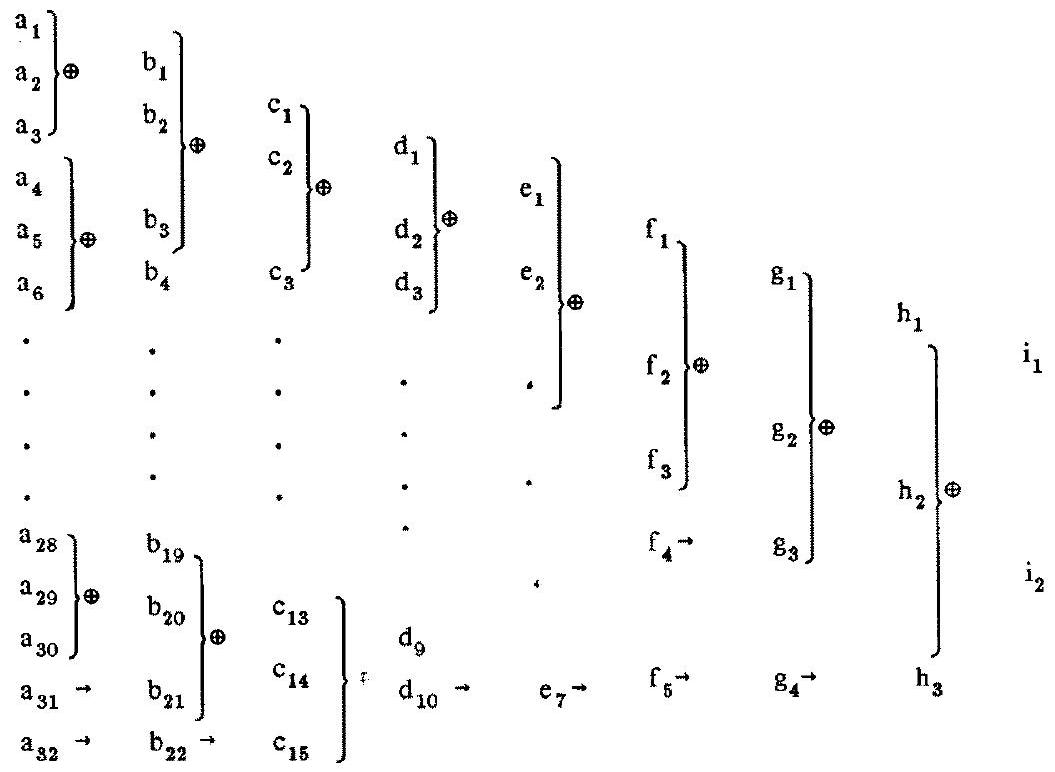
\includegraphics[alt={},max width=\textwidth]{cce78435-203d-4ce0-89c8-aaca04d3fe6b-39_772_1055_1295_144}
\end{center}
\end{figure}

For the purpose of computing timings for the various arithmetic operations, we make the following assumptions:

\begin{center}
\begin{tabular}{ll}
One CSA operation takes & a time units (t.u.) \\
One shift operation takes & b t.u. \\
One CPA operation takes & c t.u. \\
\end{tabular}
\end{center}

Furthermore we shall suppose that

$$
a \div b \quad \text { and } \quad c \div 32 a .
$$

These are reasonable assumptions since the shift can also be executed in a bit-parallel manner while the CPA must of course operate bit-serially and we are considering 32-bit words.

For the above multiplication, the terms $a_{1}, \ldots, a_{32}$ can be obtained simultaneously in $b$ t.u. Next there are eight stages of simultaneous CSA operations and finally the quantities $i_{1}$ and $\mathrm{i}_{2}$ must be added by the CPA to produce the final product. The total time for this operation is therefore $(8 a+b)+c$ t.u. which is less than $1.5 c$ t.u. The corresponding time for the ordinary "long multiplication" algorithm is 31c t.u. The potential saving is apparent.

For many of our purposes, the final CPA may be eliminated and the double number result used for the next stage of the algorithm. The multiplication of two such double numbers requires the addition of 128 terms. This requires 11 stages of simultaneous CSA operations to reduce the number of terms remaining from

128 to 86 to 58 to 39 to 26 to 18 to 12 to 8 to 6 to 4 to 3 to 2\\
and so the total time to produce the product as a double number is $11 a+b$ t.u.

The potential usefulness of these ideas within arithmetic hardware is obvious. This is explored in great detail in, for example, [35]. In the next sections we see how these advantages can be exploited in the implementation of $\ell$ i arithmetic.

\subsection*{5.3 CORDIC algorithms}
The COordinate Rotation DIgital Computer algorithms developed by Volder [63] for the evaluation of the elementary functions are based on the idea of computing $f(x)$ by decomposing the argument $x$ in the form


\begin{equation*}
x=\sum_{k=1}^{\infty} \delta_{k} \epsilon_{k} \tag{5.3.1}
\end{equation*}


where $\delta_{k}= \pm 1$ and $\Sigma \epsilon_{k}$ is a convergent series of positive terms chosen so as to combine with addition rules for $f(a \pm b)$ to yield a convenient decomposition of $f(x)$. The CORDIC algorithms use the following decomposition theorem which in this form is due to Walther [64] and Schelin [56].

Theorem 5.3.1 Suppose $\epsilon_{0} \geqslant \epsilon_{1} \geqslant \ldots \epsilon_{n}>0$ satisfy


\begin{equation*}
\epsilon_{k} \leqslant \sum_{j=k+1}^{n} \epsilon_{j}+\epsilon_{n} \quad(k=0,1, \ldots, n) \tag{5.3.2}
\end{equation*}


and let

$$
|\mathrm{r}| \leqslant \sum_{\mathrm{j}=0}^{\mathrm{n}} \epsilon_{\mathrm{j}}
$$

Define $s_{0}=0$ and $s_{k+1}=s_{k}+\delta_{k} \epsilon_{k}(k=0,1, \ldots, n)$ where $\delta_{k}=\operatorname{sgn}\left(r-s_{k}\right)$. Then


\begin{equation*}
\left|r-s_{k}\right| \leqslant \sum_{j=k}^{n} \epsilon_{j}+\epsilon_{n} \quad(k=0,1, \ldots, n+1) \tag{5.3.3}
\end{equation*}


In particular, we deduce that

$$
\left|r-s_{n+1}\right| \leqslant \epsilon_{n}
$$

Note that the choice $\epsilon_{k}=2^{-k}$ satisfies the conditions of the theorem and so any quantity $r \in[-2,2]$ can be decomposed in the form

$$
r= \pm 1 \pm 1 / 2 \pm 1 / 4 \pm \ldots \pm 2^{-n}+E
$$

where $|E| \leqslant 2^{-n}$. Thus we see that a prescribed absolute precision is obtainable with a known finite number of steps in this decomposition. Convenient addition rules exist for all the trigonometric and hyperbolic functions; these may be combined with the above theorem to yield algorithms for their evaluation. One of the major advantages of these procedures is that the computation then involves only shift and addition operations. This lack of any multiplicative operations is what gives them their speed by comparison with series or rational function approaches. Decimal versions of these algorithms are commonly employed in hand calculators for the evaluation of the elementary functions and for multiplication and division. The remarkable aspect of the CORDIC algorithm is that essentially the same algorithm with different choices of the parameters, signs and starting values achieves all of these. A general description of this algorithm follows.

\section*{CORDIC Algorithm (Binary version)}
Compute three sequences according to the recurrence relations


\begin{align*}
& x_{k+1}=x_{k}-m \delta_{k} y_{k} 2^{-k} \\
& y_{k+1}=y_{k}+\delta_{k} x_{k} 2^{-k} \\
& z_{k+1}=z_{k}-\delta_{k} \epsilon_{k} \tag{5.3.4}
\end{align*}


We use:

$$
\begin{array}{lll}
m=0 & \text { with } \epsilon_{k}=2^{-k} & \text { for multiplication and division, } \\
m=1 & \text { with } \epsilon_{k}=\tan ^{-1} 2^{-k} & \text { for the trigonometric functions, } \\
m=-1 & \text { with } \epsilon_{k}=\tanh ^{-1} 2^{-k}(k \geqslant 1) & \text { for the hyperbolic functions. }
\end{array}
$$

(Note that the equations (5.3.4) use no operations other than addition or subtraction of known constants or shifted copies of current values).

The choice of the signs $\delta_{k}$ and of the starting values depends on the individual function to be evaluated. There are two "modes" of operation - the rotation mode in which, typically, $y_{o}$ is set to zero and $\delta_{k}$ is chosen to drive $z_{k}$ toward zero by setting $\delta_{k}=\operatorname{sgn}\left(z_{k}\right)$, and the vectoring mode in which $\mathrm{z}_{0}=0$ and $\delta_{\mathrm{k}}=-\operatorname{sgn}\left(\mathrm{y}_{\mathrm{k}}\right)$. We shall consider just one example. (A more complete treatment can be found in [56] and [64].)

The third case, with $m=-1$, which is used for the hyperbolic, exponential and logarithmic functions requires a little more explanation before we proceed to the example. The choice $\epsilon_{k}=\tanh ^{-1} 2^{-k}$ does not satisfy the condition (5.3.2) of the theorem. However if the steps for $k=4,13,40, \ldots, j, 3 j+1, \ldots$ are repeated the resulting sequence $\left\{\epsilon_{k}\right\}$ is suitable.

Standard addition formulae for the hyperbolic functions yield


\begin{align*}
\cosh \left(s_{k}+\delta_{k} \epsilon_{k}\right) & =\cosh s_{k} \cosh \epsilon_{k}+\delta_{k} \sinh s_{k} \sinh \epsilon_{k} \\
& =\cosh \epsilon_{k}\left\{\cosh s_{k}+\delta_{k} \tanh \epsilon_{k} \sinh s_{k}\right\} \\
& =\cosh \epsilon_{k}\left\{\cosh s_{k}+\delta_{k} 2^{-k} \sinh s_{k}\right\} \tag{5.3.5}
\end{align*}


and similarly,


\begin{equation*}
\sinh \left(s_{k}+\delta_{k} e_{k}\right)=\cosh \epsilon_{k}\left\{\sinh s_{k}+\delta_{k} 2^{-k} \cosh s_{k}\right\} . \tag{5.3.6}
\end{equation*}


As we pointed out earlier, the number of steps of the CORDIC algorithm required to obtain a specified absolute precision is predeterminable. It follows that the factors $\cosh \epsilon_{k}$ of (5.3.5) and (5.3.6) are known in advance, as is the number of them, $N$ say. All that is necessary therefore is to store one additional constant

$$
K=\prod_{k} \cosh \epsilon_{k}
$$

where the product includes the repetitions mentioned above. The initial values $x_{1}$ and $y_{1}$ can be premultiplied by this constant so that the above relations then resemble the first two of (5.3.4) with $m=-1$. This multiplication by $K$ does not contravene the desire to use only shifts and additions since the quantities to be premultiplied are either 0 or 1 .

With the initial values $x_{1}=K, y_{1}=0$ and $\left|z_{1}\right| \leqslant \Sigma \epsilon_{k}$ and the signs $\delta_{k}$ given by $\operatorname{sgn}\left(z_{k}\right)$ the values $z_{k}$ approach zero and


\begin{equation*}
\left|z_{1}-\sum_{k=1}^{n} \delta_{k} \epsilon_{k}\right| \leqslant \epsilon_{n} \quad(n=1,2, \ldots, N) \tag{5.3.7}
\end{equation*}


while the recurrence relations (5.3.4) yield


\begin{equation*}
\left|x_{N+1}-\cosh z_{1}\right| \leqslant 2^{-N} \quad \text { and } \quad\left|y_{N+1}-\sinh z_{1}\right| \leqslant 2^{-N} . \tag{5.3.8}
\end{equation*}


\subsection*{5.4 Implementation of ai arithmetic using CORDIC algorithms}
Our primary aim here is to develop versions of the CORDIC scheme for the particular functions needed for the implementation of level-index arithmetic. The relation (5.1.3) for generating the sequence $\left(a_{j}\right)$ uses the function given by $\exp (-1 / x)$ with the argument $x$ lying in $(0,1]$. A similar function is needed to generate the sequence $\left(b_{j}\right)$.

Firstly, consider the exponential function itself. From equations (5.3.8) we see that


\begin{equation*}
x_{\mathrm{N}+1} \pm y_{\mathrm{N}+1} \div \exp \left( \pm z_{1}\right) \tag{5.4.1}
\end{equation*}


with an error not greater than $2^{-N+1}$. The recurrence relations (5.3.4) for this case are

$$
\begin{aligned}
& x_{k+1}=x_{k}+\delta_{k} y_{k} 2^{-k} \\
& y_{k+1}=y_{k}+\delta_{k} x_{k} 2^{-k} \\
& z_{k+1}=z_{k}-\delta_{k} \epsilon_{k}
\end{aligned}
$$

Adding the first two of these and denoting $x_{k}+y_{k}$ by $u_{k}$ we obtain


\begin{equation*}
u_{k+1}=u_{k}+\delta_{k} u_{k} 2^{-k} \tag{5.4.2}
\end{equation*}


which still only uses shifts and additions or subtractions to give

$$
\left|\mathrm{u}_{\mathrm{N}+1}-\exp \left(\mathrm{z}_{1}\right)\right| \leqslant 2^{-\mathrm{N}+1}
$$

for any $\left|z_{1}\right| \leqslant \sum \epsilon_{k} \div 1.13$.

But, of course, we require evaluation of quantities $\exp (-1 / x)$ and must therefore adapt this procedure to this special situation. Instead of decomposing the argument $z_{1}$ in the form $\Sigma \delta_{k} \epsilon_{k}$ as in the above algorithm, we obtain the decomposition


\begin{equation*}
-1 \div \sum \delta_{k} \epsilon_{k} x=\sum \delta_{k} \xi_{k} \tag{5.4.3}
\end{equation*}


so that

$$
-1 / x \doteq \sum \delta_{k} \epsilon_{k} .
$$

Here the new constants $\xi_{k}$. defined by $\xi_{k}=x \epsilon_{k}$, can all be computed simultaneously in an arithmetic unit with sufficient parallelism. The CORDIC-like algorithm for the function $\exp (-1 / x)$ thus becomes:


\begin{align*}
& u_{1}=K, \quad v_{1}=1 \\
& \delta_{k}=-\operatorname{sgn}\left(v_{k}\right)  \tag{5.4.4}\\
& u_{k+1}=u_{k}+\delta_{k} u_{k} 2^{-k} \\
& v_{k+1}=v_{k}+\delta_{k} \xi_{k}
\end{align*}


For the sequence $\left\{b_{j}\right\}$ the recurrence relation relies on evaluations of the function $\exp ((y-1) / x)$. This is achieved by simply setting

$$
v_{1}=1-y
$$

in the algorithm defined by equations (5.4.4).

There is a serious and obvious drawback to this algorithm as we have it thus far. The restriction of the range to $\left|z_{1}\right| \leqslant 1.13$ implies that the above algorithm is only useful for $|x| \geqslant 1 / 1.13$ and since we have $0<x \leqslant 1$ we clearly must extend this range. This extension of the range is a common problem for elementary function routines. In this case the inclusion of two additional steps using $\epsilon_{1}=\tanh ^{-1} 1 / 2 \doteqdot 0.549$ extends the range of the original algorithm to $\left|z_{1}\right| \leqslant 2.228$ and therefore the range for $x$ above to $x \geqslant 0.45$.

Now the analyses of the $\Omega i$ arithmetic algorithms [9,10] show that (for single precision working) the values $a_{j}$ are required to an absolute precision of $2^{-37}$. For any $x<2^{-5}$ we have


\begin{equation*}
\exp (-1 / x)<e^{-32}<2^{-46}=0 ; \operatorname{ap}\left(2^{-37}\right) \tag{5.4.5}
\end{equation*}


so that if $\mathrm{a}_{\mathrm{j}}<1 / 32$ we simply return the value $\mathrm{a}_{\mathrm{j}-1}=0$. If $\mathrm{x} \geqslant 1 / 32$ then doubling x at most four times results in an argument greater than $1 / 2$ and so within the range of our algorithm. This is compensated by squaring the result the same number of times since

$$
\exp (-1 / x)=(\exp (-1 / 2 x))^{2}
$$

We turn now to considerations of the operation time for computation of the sequence $\left\{\mathrm{a}_{\mathrm{j}}\right\}$ using this approach in combination with the "double-number" philosophy discussed in Section 5.2. First, we must compute $\mathrm{a}_{\ell-1}=\mathrm{e}^{-\mathrm{f}}$ as a double number with the required accuracy $2^{-37}$. This needs 39 steps of the CORDIC algorithm allowing for the necessary repetitions. (Note that there is no range extension needed for this part of the calculation). Thus we set

$$
u_{1}=K, \quad v_{i}=f, \quad \delta_{k}=\operatorname{sgn}\left(v_{k}\right)
$$

and, in parallel with each other,

$$
u_{k+1}=u_{k}-\delta_{k} u_{k} 2^{-k} \quad \text { and } \quad v_{k+1}=v_{k}-\delta_{k} \epsilon_{k}
$$

For $k>1$ the choice of $\delta_{k}$ involves finding the sign of a double number. We assume this operation takes $d$ t.u. Each of the parallel steps takes $2 a+b$ t.u. since the $u_{k}$ are double numbers. Hence the total time for this stage is $39(2 a+b+d)$ t.u.

For the computation of $\mathrm{a}_{\mathrm{j}-1}$ from $\mathrm{a}_{\mathrm{j}}$, we have a maximum of four "doublings" of $\mathrm{a}_{\mathrm{j}}$ to obtain the argument $x>0.45$. This takes a maximum of $4 b$ t.u. since multiplication by 2 is simply a shift of one place. Next the quantities $\left\{\xi_{k}\right\}$ are obtained as double numbers by parallel multiplication of the stored single-number constants $\left\{\epsilon_{k}\right\}$ by $x$. This step takes $(10 \mathrm{a}+\mathrm{b})$ t.u. The necessary 41 steps of CORDIC algorithm are accomplished in $41(2 a+b+d)$ t.u. and must be followed by up to four "squarings" of the result. These "double $x$ double" multiplications take $12 a+b$ t.u. each. The maximum time for computing $a_{j-1}$ from $a_{j}$ is therefore

$$
140 a+50 b+41 d \text { t.u. }
$$

With a simple modification of the way in which the sequence $\left\{\mathrm{b}_{\mathrm{j}}\right\}$ is started this can be computed in parallel with the $\left\{\mathrm{a}_{\mathrm{j}}\right\}$ in the same time.

The recurrence relation for the sequence $\left\{c_{j}\right\}$ can be implemented with the standard CORDIC algorithm for the logarithm function modified to use the constants

$$
\alpha_{k}=a \epsilon_{k}
$$

in order to evaluate the function a $x$ In $c$. Again some initial scaling is required but this is readily accomplished. (A complete treatment of this and the timings involved can be found in [61]).

The overall times for this operation are critically dependent on the time, d, needed for obtaining the sign of a double number. In Section 5.6 we discuss and compare these times with those of the table look-up approach of the next section. For a "typical" case where the levels of both $x$ and $z$ are 3 , we find that this operation time ranges from about twice to six or seven times that of a floating-point long-multiplication as $d$ varies from about $2 a$ to about 16a.

\subsection*{5.5 The table look-up approach}
In this section we turn to a different approach to the implementation of level-index arithmetic in which the double number philosophy is combined with a partial table look-up scheme. The idea is to use several small tables for the appropriate exponential functions. The argument is divided up into subwords corresponding to the various tables which can then be consulted simultancously.

Consider first the computation of $\mathrm{a}_{\mathrm{j}-1}$ to the required working precision of $2^{-37}$. For this approach this calculation has two stages the first of which is the efficient reciprocation of $a_{j}$ We require


\begin{equation*}
t=1 / a_{j} ; \quad \operatorname{ap}\left(2^{-37}\right) . \tag{5.5.1}
\end{equation*}


By (5.4.5) we may again deduce that

$$
a_{j} \leqslant 1 / 32 \Rightarrow a_{j-1} \approx 0 ; \operatorname{ap}\left(2^{-37}\right)
$$

and hence $t<32$. Storage of $t$ thus requires 42 bits including five before the binary point. To facilitate the reciprocation, we first shift $a_{j}$ to the interval $[1 / 2,1)$ and subtract the result from unity so that we seek $1 /(1-\delta)$ with $\delta \epsilon(0,1 / 2]$. (Of course, in forming $t$ we must shift the result the appropriate number of places to compensate for this initial shift. This has been accounted for in the timings below).

The necessary accuracy in $1 /(1-\delta)$ can be obtained from the geometric series using the terms

$$
1+\delta+\delta^{2}+\ldots+\delta^{41}
$$

(Alternatively, we may use the approximation

$$
1 /(1-\delta) \div(1+\delta)\left(1+\delta^{2}\right)\left(1+\delta^{4}\right) \ldots\left(1+\delta^{32}\right)
$$

which may achieve a further marginal speed-up.) Now, obtaining $\delta$ consists of a shift and the forming of the two's complement. We assume the latter takes the same time $b$ t.u. so that finding $\delta$ takes 2 b t.u. Next we form $\delta^{2}$ as a double number; this takes a further $8 \mathrm{a}+\mathrm{b}$ t.u.

For the remaining powers of $\delta$, parallel computation yields significant gains. For $k= 1,2,3,4,5$, we can form $8^{2^{\mathbf{k}}+1} \ldots, 8^{2^{\mathbf{k}+1}}$ as double numbers in parallel. Each such stage takes $12 a+b$ t.u.

There are now 40 double and two single numbers to be summed and, finally, shifted to form $t$ as a single number. This part of the operation takes $10 a+b+c$ t.u. which yields a total time for the reciprocation of

$$
78 a+10 b+c \text { t.u. }
$$

Note that further slight gains can be achieved by forming some of the partial sums simultaneously with the computation of the next group of terms in the expansion.

To complete the calculation of $\mathrm{a}_{\mathrm{j}-1}$ we must evaluate $\mathrm{e}^{-\mathrm{t}}$. Write


\begin{equation*}
t=t_{1}+t_{2}+\ldots+t_{7} \tag{5.5.2}
\end{equation*}


where each $t_{i}$ is the $i^{\text {th }}$ 6-bit subword of the 42-bit word $t$. This can be achieved by simultaneous shift operations and takes b t.u. We can now use parallel table look-up for the values $\exp \left(-t_{i}\right)$, and we shall assume that this look-up operation takes e t.u.

There are now seven factors to be multiplied. This can be accomplished using a tree of parallel multiplications each of which makes maximal use of the CSA and double numbers.\\
The time for this part of the calculation is

$$
32 a+3 b+c \text { t.u. }
$$

and so the total time for the computation of $\mathrm{a}_{\mathrm{j}-1}$ from $\mathrm{a}_{\mathrm{j}}$ is

$$
110 a+14 b+2 c+e \text { t.u. }
$$

In parallel with this calculation we can compute $b_{j-1}$ using $a_{j}$ and $b_{j}$ with just a small time-lag caused by the need to compute

$$
t^{\prime}=\left(1-b_{j}\right) t .
$$

This multiplication requires $10 a+b$ t.u. and so assuming that $e>10 a+b$, we can compute $\mathrm{a}_{\mathrm{j}-1}$ and $\mathrm{b}_{\mathrm{j}-1}$ in

$$
110 a+14 b+2 c+2 e \text { t.u. }
$$

The calculation of $\mathrm{a}_{\ell-1}$ ( and , perhaps, $\mathrm{b}_{\ell-1}$ ) is a much quicker process for the table look-up approach since no reciprocation step is needed. This can be achieved in

$$
32 a+4 b+c+2 e+\max (c, e) \quad \text { t.u }
$$

Full details can be found in [52].

For the computation of the sequence $\left\{c_{j}\right\}$ using the recurrence relation

$$
c_{j+1}=1+a_{j+1} \ln c_{j}
$$

we begin by forming $c_{0}=1 \pm b_{0}$ which entails either the insertion of a $l$ before the binary point or the taking of the two's complement of $b_{0}$. This operation takes $b$ t.u. Write


\begin{equation*}
c_{j}=s(1+\sigma) \tag{5.5.3}
\end{equation*}


where $s$ comprises the first six significant bits of $c_{\mathbf{j}}$. It follows that

$$
\sigma<2^{-5} .
$$

Dividing $c_{j}$ by $s$ using a similar approach to the reciprocation above, we can obtain $\sigma$ to the required absolute precision of $2^{-32}$ in a total of $57 a+b$ t.u.

Since $\sigma<2^{-5}$, the necessary accuracy for $\ln (1+\sigma)$ can be obtained from the approximation

$$
\sigma-\sigma^{2} / 2+\sigma^{3} / 3-\sigma^{4} / 4+\sigma^{5} / 5 .
$$

The terms of this expansion can now be computed in three stages as follows: first $\sigma^{2}, \sigma / 3$ and $\sigma / 5$ are computed as double numbers; from these $\sigma^{3} / 3$ and $\sigma^{4}$ and then, finally, $\sigma^{5} / 5$, $\sigma^{2} / 2$ and $\sigma^{4} / 4$ can be obtained. Each of these steps takes $12 a+b$ t.u.

This leaves nine terms to be added together with 1 n s . This last term is obtained by table look-up taking account of the initial shift required to obtain the leading six significant bits. The total time to produce $\ln c_{j}$ is therefore $98 a+11 b$ t.u and hence we may deduce that the overall time required for computing $c_{j+1}$ is

$$
109 a+12 b+c \text { t.u. }
$$

In this timing we have assumed that the table look-up time for the six bit table, e t.u., does not exceed $100 \mathrm{a} \div 3 \mathrm{c}$ t.u. and therefore that $\ln \mathrm{s}$ can be obtained simultaneously with the rest of the calculation described above.

In the next section we compare the timings for the implementation of the $\ell$ arithmetic algorithms adopting this approach with those for the CORDIC techniques. The assumptions made for the table look-up time bracket this between (approximately) $c / 3$ and $3 c$ and, for this range of values of $e$, we find that "typical" arithmetic times are of the order of twice those of floating-point long multiplications.

In this case it is also necessary to address the question of the storage requirement of the tables suggested. For the sequence $\left(\mathrm{a}_{\mathrm{j}}\right)$ and $\left(\mathrm{b}_{\mathrm{j}}\right)$ we need seven tables, each with $2^{6}=64$ entries, while for $\left\{c_{j}\right\}$ only one such table is necessary. In total therefore, some 512 entries each of substantially fewer than 60 bits would be needed. A generous upper bound for the storage requirement is thus around 30,000 bits which would occupy only a small corner of a level-index arithmetic chip. The feasibility of on-chip storage of the tables renders the table look-up times cited above attainable.

\subsection*{5.6 Overall arithmetic times and conclusions}
The steps needed to complete the $\ell$ i arithmetic algorithms can be accomplished in essentially the same ways as have been described in the preceding sections.

For subtraction when $n<\ell$, that is when the level of the result $z$ is less than that of $x$, a single division is required. For the case $n=\ell$ and for addition the quantity $f+\ln c_{\ell-1}$ must be computed. The addition algorithm may require yet one further logarithm. Whether the CORDIC or the table look-up approach is to be adopted these final stages can be readily accomplished with minor variations - often simplifications - of the procedures already described.

The "worst case" for which level-index arithmetic ever need be performed is with $\ell=m=n=5$ since all arithmetic beyond that level is trivial in the sense discussed elsewhere in this course. The overall time for the CORDIC implementation for this case is

$$
C_{1}=1168 a+467 b+c+409 d \text { t.u }
$$

while for the table look-up method it is

$$
L_{1}=1006 a+120 b+14 c+9 e+\max (c, e) \text { t.u. }
$$

The major attraction of the CORDIC scheme is the retention of the double numbers throughout the calculation to the extent that only one CPA operation is used. The associated cost is plain - the coefficient of $d$ is large. The dependence of the table look-up method on $e$ is less critical. Under the assumptions made earlier that

$$
a \div b \div c / 32
$$

these times are given by

$$
C_{1} \doteqdot 52 c+409 d \quad \text { and } \quad L_{1} \div 49 c+9 e+\max (c, e)
$$

For a more realistic assessment of the potential of these implementations which is not unfairly favourable to the $\ell$ i system consider a "typical" operation with $\ell=n=3$. The corresponding times are then

$$
C_{2}=722 a+293 b+c+259 d \div 33 c+259 d \text { t.u. }
$$

and

$$
L_{2}=568 a+68 b+8 c+6 e+\max (c, e) \div 28 c+6 e+\max (c, e) t u .
$$

Single precision floating-point long multiplication would be expected to take of the order of 25 c t.u. and it is this figure which is used in the following table to estimate level-index times in terms of floating-point multiplications, fpm.

\begin{table}[h]
\begin{center}
\captionsetup{labelformat=empty}
\caption{TABLE 5.5.1}
\begin{tabular}{|l|l|l|l|l|l|}
\hline
\multicolumn{3}{|c|}{CORDIC} & \multicolumn{3}{|c|}{Table look-up} \\
\hline
d & Typical time & Worst case time & e & Typical time & Worst case time \\
\hline
2a or c/16 & 49c or 2 fpm & 77c or 3 fpm & 11a or c/3 & 34 c or 1.5 fpm & 53c or 2 fpm \\
\hline
4 a or c/8 & 65c or 2.5 fpm & 103c or 4fpm & 32a or c & 37 c or 1.5 fpm & 59c or 2.5 fpm \\
\hline
8a or c/4 & 98c or 4 fpm & 154c or 6 fpm & 96a or 3c & 47 c or 2 fpm & 79c or 3 fpm \\
\hline
\end{tabular}
\end{center}
\end{table}

It would be unwise at this stage to draw firm conclusions as to what will be the best way in which to implement $2 i$ arithmetic. What can be safely concluded from the study of these approaches is that it will be possible to implement it in ways which will not be much slower than floating-point computation. The final implementation may well use combinations of all the ideas considered here and others too. The surface-fitting approach to be considered in the final lecture of this series is also highly promising.

It is relevant to point out here that the evidence of Sweeney [58] is that only a very small proportion of computer run-time is spent on floating-point operations even within large scientific computing programs. Thus the effect of slowing down the arithmetic operations themselves is much diluted in its effect on run-times. In combination with the fact that a robust arithmetic system will allow much simpler programs to be used, the overall effect on program development and run times is likely to be beneficial.

\section*{6: APPLICATIONS}
\section*{C.W.Clenshaw}
\subsection*{6.1 Introduction}
In this lecture we examine the results obtained from the application of sli arithmetic to two particular problems in numerical analysis. Programs were prepared for the VAX at Lancaster and for the UNIVAC at the NBS, based on software implementations of the algorithms already described. These implementations use flp arithmetic internally, and they also use standard machine routines for the exponential and logarithmic functions. Thus they are slow, and they are not amenable to the kind of error analyses which we explored in [9] and [10]. Nevertheless, they are genuine sqi programs, in the sense that their results will be similar to those produced by a fully polished sti implementation which has similar limitations of precision. Since our first aim is to confirm the practical usefulness of sti, we now apply these programs to (i) the calculation of the binomial probability distribution; (ii) the solution of real polynomial equations by Graeffe's method of root squaring.

\subsection*{6.2 The binomial probability distribution}
The function which we wish to calculate is defined by

$$
I(n, r, p)=\sum_{S=0}^{r}\binom{n}{s} p^{s} q^{n-s}
$$

where $q=1-p, 0 \leqslant p \leqslant 1,0 \leqslant r \leqslant n$.

The problems associated with magnitude here are well known, and widely discussed in the literature. If calculation is undertaken directly in flp, the numerator and denominator of $\left[\begin{array}{l}n \\ s\end{array}\right]$ overflow, and $p^{s}$ and $q^{n-s}$ underflow, for quite moderate values of the parameters, even though the resulting I always lies between 0 and 1.

It is possible to overcome the difficulties by careful analysis and scaling, but the resulting algorithm is inevitably somewhat complicated. Sterbenz [57] devotes several pages to this problem. In contrast, we can implement almost any algorithm, however simple, in s $\ell$. For example, given $p, n$, and $r$, we might first evaluate

$$
\mathrm{q}^{\mathrm{n}}=\mathrm{q} \times \mathrm{q} \times \mathrm{q} \times \mathrm{q} \ldots
$$

Then for each $s$ from 1 to $n$ form

$$
\begin{aligned}
n!/(n-s)! & =(n!/(n-s+1)!) \times(n-s+1) \\
s! & =(s-1)!\times s \\
p^{s} & =p^{\beta-1} \times p \\
q^{n-s} & =q^{n-(s-1)} / q
\end{aligned}
$$

following which each term of the sum can be calculated directly, and I found by summation.

In the case $\mathrm{p}=0.1, \mathrm{n}=2000, \mathrm{r}=200$ (which is used by Sterbenz) we find, for the last term in the sum, the values

$$
\begin{aligned}
n \times(n-1) \times & \ldots \times(n-T+1)=\phi(4.68842667) \\
r! & =\phi(4.64769156) \\
p^{r} & =1 / \phi(4.59530170) \\
q^{n-r} & =1 / \phi(4.50519488)
\end{aligned}
$$

Then

$$
\left[\begin{array}{l}
\mathrm{n} \\
\mathrm{r}
\end{array}\right] \mathrm{p}^{\mathrm{r}} \mathrm{q}^{\mathrm{n} \sim \mathrm{r}}=1 / \phi(3.22893 \text { 471 })
$$

and we find, on adding this to the other similarly-calculated terms,

$$
\mathrm{I}=1 / \phi(1.65619393)=0.51882226
$$

There is some loss of accuracy here through cancellation (the correct 8D result is 0.51882040 ) but we clearly have a useful result, even in this rather extreme case. (We may note, for example, that $\phi(4.6) \div 6.3 \times 10^{210}$ while $\phi(4.7) \div 3 \times 10^{778}$ ).

This loss is interesting: it tends to provoke a quick reaction from flp defenders who will say that this is evidence that sei is subject to loss of precision in circumstances where flp cannot lose precision. We have performed multiplications and divisions, followed by addition of positive quantities. There has been no subtraction, so there can be no cancellation.

This plausible-sounding argument is based upon the assumption that the proper measure of precision is relative precision. As we have already seen, this is not the case for large numbers. When we divide two such numbers there is cancellation in the exponent, and information is lost. If the above example could be carried out by the same method in flp (which is not possible for any existing orthodox system) then it would suffer similar cancellation.

Not least of the advantages of $\ell i$ and $s \ell i$ is that they make manifest some properties of ordinary arithmetic operations that are concealed by flp; in this case, the essential similarity of the nature of subtraction and division from the standpoint of precision.

\subsection*{6.3 Root squaring}
Graeffe's method of root squaring for the solution of polynomial equations presents greater difficulties because the very large (or very small) numbers which occur naturally in its execution are much more difficult to remove by scaling. Nevertheless, the theoretical attractions of the method are such that in pre-computer days, when the result of each arithmetic operation could be observed and acted upon, root squaring featured prominently in the literature. Up until the 1960's many books on numerical analysis included an account of root squaring (among them Hildebrand [31] and Ralston [55]) and a comprehensive description of its implementation on desk machines was given by Olver [47]. In 1960 Bareiss [1] showed how a computer might be programmed to perform root squaring, and more recently, a discussion of this method appeared in Henrici [30]. Generally speaking, however, numerical analysts have sought methods which are more readily programmable. The attractive simplicity of the root-squaring method tends to be lost in the devices needed to avoid catastrophic overflow and underflow in a flp system.

Thus this method is an obvious test vehicle for any new system of arithmetic which claims to free computations from these phenomena. We now give a very brief outline of the method. Suppose that the polynomial whose zeros are required is given by


\begin{equation*}
p(z)=K\left(z-\alpha_{1}\right) \quad\left(z-\alpha_{2}\right) \quad\left(z-\alpha_{3}\right) \ldots\left(z-\alpha_{n}\right) . \tag{6.3.1}
\end{equation*}


Then

$$
(-1)^{n} p(z) p(-z)=K\left(z^{2}-\alpha_{1}^{2}\right)\left(z^{2}-\alpha_{2}^{2}\right) \ldots\left(z^{2}-\alpha_{n}^{2}\right),
$$

so the multiplication of $p(z)$ by $p(-z)$ gives a new polynomial whose zeros are the squares of those of the original. This process may be repeated as often as we wish.\\
We write


\begin{align*}
& f_{0}(z)=p(z) \\
& f_{r+1}\left(z^{2}\right)=(-1)^{n} f_{r}(z) f_{r}(-z), \quad r=0,1,2, \ldots \tag{6.3.2}
\end{align*}


with


\begin{equation*}
f_{r}(z)=\sum_{j=0}^{n}(-1)^{n-j} a_{j}^{(r)} z^{j} \tag{6.3.3}
\end{equation*}


Substitution of (6.3.3) in (6.3.2) gives


\begin{equation*}
a_{j}^{(r+1)}=\left(a_{j}^{(r)}\right)^{2}+2 \sum_{k=1}^{\min (j, n-j)}(-1)^{k_{a}(r)} a_{j+k}^{(r)} \tag{6.3.4}
\end{equation*}


The mechanical process of root squaring is therefore very simple. What it achieves is, of course, the increased separation of real, distinct zeros (we shall see what happens to other types of zero later) to the point at which they can be deduced very easily from the coefficients.

For simplicity, let us examine a cubic.

Let $\alpha_{1}, \alpha_{2}$ and $\alpha_{3}$ be the real zeros of

$$
f_{0}(z)=p(z)=a_{3}^{(0)} z^{3}-a_{2}^{(0)} z^{2}+a_{1}^{(0)} z-a_{0}^{(0)}
$$

and let us, for the sake of brevity, denote by $t_{1}, t_{2}$ and $t_{3}$ the zeros of

$$
f_{r}(z)=a_{3}^{(r)} z^{3}-a_{2}^{(r)} z^{2}+a_{1}^{(r)} z-a_{0}^{(r)} .
$$

(Thus we have $t_{j}=\alpha_{j}^{2^{r}}$ ).

The ratios of successive coefficients yield

$$
\begin{aligned}
& \frac{a_{2}^{(r)}}{a_{3}^{(r)}}=t_{1}+t_{2}+t_{3} \\
& \frac{a_{1}^{(r)}}{a_{2}^{(r)}}=\frac{t_{1} t_{2}+t_{1} t_{3}+t_{2} t_{3}}{t_{1}+t_{2}+t_{3}} \\
& \frac{a_{0}^{(r)}}{a_{1}^{(r)}}=\frac{t_{1} t_{2} t_{3}}{t_{1} t_{2}+t_{1} t_{3}+t_{2} t_{3}}
\end{aligned}
$$

If $\left|t_{1}\right| \gg\left|t_{2}\right| \gg\left|t_{3}\right|$, these are approximately $t_{1}, t_{2}$ and $t_{3}$ respectively. If $r$ is large enough for the separation of zeros to be acceptable, then we can then recover the wanted $\alpha_{\mathrm{j}}$ by\\
taking the appropriate root of $t_{j}$ (except that the sign will be undetermined as yet, since this will have been lost in the first squaring).

So in all cases we define

$$
\alpha_{j}^{(r)}=\left|a_{n-j}^{(r)} / a_{n-j+1}^{(r)}\right|^{2^{-r}}
$$

If $\left|\alpha_{1}\right|>\left|\alpha_{2}\right|>\left|\alpha_{3}\right| \ldots$ then $\alpha_{j}^{(r)} \rightarrow\left|\alpha_{j}\right|$ as $r \rightarrow \infty$.

As a simple example, consider the cubic $z^{3}-6 z^{2}+11 z-6$. In this case we find (to 5D)

$$
\begin{array}{ll}
\alpha_{1}^{(0)}=6 & \\
\alpha_{1}^{(1)}=14^{2^{-1}} & =3.74166 \\
\alpha_{1}^{(2)}=98^{2^{-2}} & =3.14635 \\
\alpha_{1}^{(3)}=6818^{2^{-3}} & =3.01444 \\
\alpha_{2}^{(0)}=11 / 6 & =1.83333 \\
\alpha_{2}^{(1)}=(49 / 14)^{2^{-1}} & =1.87083 \\
\alpha_{2}^{(2)}=(1393 / 98)^{2^{-2}} & =1.94170 \\
\alpha_{2}^{(3)}=(1686433 / 6818)^{2^{-3}} & =1.99143 \\
\alpha_{3}^{(0)}=6 / 11 & \\
\alpha_{3}^{(1)}=(36 / 49)^{2^{-1}} & =0.54545 \\
\alpha_{3}^{(2)}=(1296 / 1393)^{2-2} & =0.85714 \\
\alpha_{3}^{(3)}=(1679616 / 1686433)^{2^{-3}} & =0.98212
\end{array}
$$

Further similar cycles of the squaring process will demonstrate rapid convergence of the three sequences to the limits 3, 2 and 1 respectively.

Several questions are raised at once: for example\\
(i) How do we determine the sign of each real zero?\\
(ii) What happens when not all zeros are well separated? (In particular, how are complex zeros and repeated zeros determined?)\\
(iii) How do we deal with the large numbers, and the consequent large errors, that appear after only a few cycles?

The first two questions are readily answered. When a real zero has been isolated, we simply calculate $p\left( \pm \alpha_{k}\right)$; the magnitude of the two residuals will indicate which is the correct sign.

Now suppose that two dominant zeros of the cubic share the same modulus $|\alpha|$, and let us write the zeros of $f_{r}(z)$ as

$$
t_{1}=p e^{i \theta}, t_{2}=p e^{-i \theta}, t_{3}
$$

In this case we have

$$
\begin{aligned}
& \alpha_{1}^{(r)}=\left|2 p \cos \theta+t_{3}\right|^{2^{-r}} \rightarrow|2 p \cos \theta|^{2^{-r}} \text { if } \cos \theta \neq 0, \\
& \alpha_{2}^{(r)}=\left|\frac{p^{2}+2 p t_{3} \cos \theta}{2 p \cos \theta+t_{3}}\right|^{2^{-r}} \rightarrow\left|\frac{p}{2 \cos \theta}\right|^{2^{-r}} \\
& \alpha_{3}^{(r)}=\left|\frac{p^{2} t_{3}}{p^{2}+2 p t_{3} \cos \theta}\right|^{2^{-r}} \rightarrow t_{3}^{2^{-r}} \rightarrow\left|\alpha_{3}\right| .
\end{aligned}
$$

We see that the distinct root is still exposed as before, but that the pair has become relatively complicated. However, if we define

$$
\beta_{j}^{(r)}=\left[\begin{array}{cc}
\alpha_{j}^{(r)} & \alpha_{j-1}^{(r)}
\end{array}\right]^{1 / 2}
$$

we see that here $\beta_{2}^{(r)} \rightarrow \mathrm{p}^{2^{-r}} \rightarrow|\alpha|$, so the modulus of the pair is exposed by the $\beta$-sequence just as is that of the real root by the $\alpha$-sequence.

In solving an arbitary polynomial equation with real coefficients, we must expect real roots and complex conjugate pairs; higher multiplicities are much less common. We therefore envisage a standard output from a root-squaring program which will give values of $\alpha_{j}^{(r)}$ and $\beta_{j}^{(r)}$, together with the residuals $p\left( \pm \alpha_{j}^{(r)}\right)$ and $p\left( \pm \beta_{j}^{(r)}\right)$. These should serve to identify isolated real zeros, and pairs of zeros sharing the same modulus. (A pair may be complex conjugates, real and equal, or real and equal-opposite).

\subsection*{6.4 Precision}
It is easy to appreciate that for even quite moderate values of $r$, the coefficients in $f_{r}(z)$ will be subject to large relative errors. (In our example above, the coefficents were exact for $\mathbf{r}=0,1,2,3$, but even here their sheer magnitude will force rounding, and therefore rounding errors, in succeeding cycles). These errors grow so rapidly that there may soon be no correct significant figures in the $\mathbf{a}_{\mathbf{j}}^{(r)}$. However, this is not in itself a matter for\\
concern; the information that is apparently lost in the process of root squaring is patently recovered in the calculation of the $\alpha_{j}$. This phenomenon is described more fully in [11]: see also [44], and Olver's Lecture 4.

It is important to notice that we have not yet invoked sli arithmetic. We have merely observed that relative error is an inappropriate measure for calculations of this nature, where results of moderate magnitude are extracted from intermediate calculations where numbers may be very large (or small). We now note that the use of sli arithmetic, and the naturally associated notion of generalized precision, enables this problem to be treated without difficulty.

\subsection*{6.5 The application of sli to root squaring}
In [11] we give an account of the results obtained when a simple implementation of sli is applied directly to four separate polynomials of widely differing nature. Here we merely sketch the salient points, and describe some results from just two of those problems.

We have used sli (rather than $\ell i$ ) in order that we need not address the problem of scaling. It is true that, whether we use 2 i or sli, the simple multiplication of the coefficients of a polynomial by a constant will affect the conditioning of the problem of root-finding, and there is some interest in determining the optimal scaling procedure of this kind. However, our present purpose is to investigate the efficacy of level-index arithmetic in dealing with magnitude and precision in extreme circumstances; we therefore proceed with an algorithm which is immediately applicable to any polynomial with real coefficients, even though end-figure errors may be larger than necessary.

The calculation of the phase of complex zeros also raises questions which, for similar reasons, we shall not pursue here. Our aim will be to calculate the modulus of each zero, and we shall incidentally determine (in most cases) whether it is real or complex. In the case of real zeros, we shall determine their signs also.

The routine used is a straightforward implementation in sli of the algorithm described in Section 6.3. (This implementation uses double-precision floating-point arithmetic internally, and yields a gp of about $10^{-13}$ where there is no cancellation.) The output after each iterative cycle consists of the four vectors mentioned above; it contains the information that will in general yield on inspection the required distinct real zeros, and the moduli of complex zeros (as well as the equal/opposite real pairs). Higher multiplicities may not be revealed at once. However, their occurrence should be rare, and in any case it is not difficult to extract them once their presence is suspected. (See [11] for further details, including a more detailed presentation of numerical results.)

The first example which we present here is a simple one used by Matsui and Iri [45]. It is a polynomial of degree four, given by

$$
p(x)=x^{4}-a_{3} x^{3}+a_{2} x^{2}-a_{3} x+a_{0}
$$

where

$$
\begin{array}{llll}
a_{3}=10.43857 & 59302 & 0614 & a_{1}=69.60408 \\
a_{2}=40.58740 & 56758 & 7410 & a_{0}=44.36715 \\
a_{2} & 61490 & 6059
\end{array} .
$$

This is fairly ill conditioned problem: to 14D the smallest zero is 2, the largest is 3, and the other two are the rounded values of $e$ and $\sqrt{ }(7.4)$, namely\\
2.71828182845904 and 2.72029410175647\\
respectively.

It transpires that after 15 cycles the $\alpha$-values in the first output vector have settled to within a unit or two in the 14th decimal place. We give below the approximations to the sccond largest zcro for iterations 14 through 17.

\begin{center}
\begin{tabular}{llll}
Iteration &  & Approximation &  \\
\cline { 3 - 3 }\cline { 4 - 4 }
14 &  &  &  \\
15 &  & 2.72029 & 41026 \\
16 &  & 3166 &  \\
17 &  & 2.72029 & 41017 \\
17 &  & 3066 &  \\
 &  & 2.72029 & 41017 \\
 &  & 3064 &  \\
 &  & 3065 &  \\
\end{tabular}
\end{center}

The approximation is remarkably stable - after 50 cycles we obtain the value 2.72029410173055 - but it is clear that stability is no guarantee of accuracy. In this case the ill-conditioning overlaying the limited precision of the arithmetic is sufficient to cause the loss of the last four figures given. (The other three zeros are similarly indicated, but with rather greater accuracy: the second zero is the worst conditioned).

We may note that in this example, which is by no means an extreme one, our computation has dealt with numbers that are very large by conventional standards. After $r$ cycles the coefficient $\mathrm{a}_{3}{ }^{(\mathrm{r})}$ exceeds $3^{2^{\mathrm{r}}}$, since all the zeros are positive. With $\mathrm{n}=15$ this is about $2 \times 10^{15634}$. (The value with $n=50$, where we examined meaningful results, exceeds $10^{10^{14}}$ ).

Our second example, also treated at greater length in [11], is a polynomial of degree 14 with zeros of varying character. It is given by

\begin{table}[h]
\begin{center}
\begin{tabular}{|l|l|l|l|l|l|l|}
\hline
k & $\alpha_{k}^{(10)}$ & $p\left(t \alpha_{k}^{(10)}\right)$ &  & $B_{k}^{(10)}$ & $p\left( \pm \beta_{k}^{(10)}\right)$ &  \\
\hline
\multirow[t]{2}{*}{1} & \multirow[t]{2}{*}{2.31237647787152} & [4.01576326389222] & 1 &  &  &  \\
\hline
 &  & [3.90307296757064] & -1 &  &  &  \\
\hline
\multirow[t]{2}{*}{2} & \multirow[t]{2}{*}{1.95977873402839} & [3.91434499764033] & 1 & 2.12878985491760 & [3.97360414323500] & 1 \\
\hline
 &  & [3.927902060761220] & 1 &  & [-3.96974834023348] & 1 \\
\hline
\multirow[t]{2}{*}{3} & \multirow[t]{2}{*}{2.00016078777021} & [3.93137606887548] & 1 & 1.97986680777004 & [3.92311703703905] & 1 \\
\hline
 &  & [-3.67512474462557] & 1 &  & [3.90713538488153] & 1 \\
\hline
\multirow[t]{2}{*}{4} & \multirow[t]{2}{*}{2.04088266744541} & [3.94641513170820] & 1 & 2.02041913569046 & [3.93909242828714] & 1 \\
\hline
 &  & [-3.93444724555156] & 1 &  & [-3.91089253762885] & 1 \\
\hline
\multirow[t]{2}{*}{5} & \multirow[t]{2}{*}{1.66779521821806} & [2.33112195692192] & -1 & 1.84493207292560 & [3.84646463238930] & 1 \\
\hline
 &  & [3.95029146536699] & 1 &  & [3.9558596726904] & 1 \\
\hline
\multirow[t]{2}{*}{6} & \multirow[t]{2}{*}{1.66553887877075} & [2.34854857504526] & -1 & 1.66666666666437 & [4.06921586867569] & -1 \\
\hline
 &  & [3.95004512185302] & 1 &  & [3.95016880628101] & 1 \\
\hline
\multirow[t]{2}{*}{7} & \multirow[t]{2}{*}{1.41517116999438} & [2.66976438637781] & 1 & 1.53525978379593 & [3.62559718897801] & 1 \\
\hline
 &  & [3.69800654487441] & 1 &  & [3.92587594535703] & 1 \\
\hline
\multirow[t]{2}{*}{8} & \multirow[t]{2}{*}{1.41325660274334} & [-2.66799164372710] & 1 & 1.41421356237542 & [4.05673599717207] & -1 \\
\hline
 &  & [-3.69772407136798] & 1 &  & [3.92261804103378] & -1 \\
\hline
\multirow[t]{2}{*}{9} & \multirow[t]{2}{*}{1.20126536676056} & [-4.08922902562647] & -1 & 1.30295671885956 & [-3.59769879290383] & 1 \\
\hline
 &  & [-3.92213072487545] & 1 &  & [-3.90946181799193] & 1 \\
\hline
\multirow[t]{2}{*}{10} & \multirow[t]{2}{*}{1.00000000000000} & [3.70533444232518] & 1 & 1.09602252110099 & [3.66550681884250] & 1 \\
\hline
 &  & [-3.92358170908464] & 1 &  & [-3.92504514072812] & 1 \\
\hline
\multirow[t]{2}{*}{11} & \multirow[t]{2}{*}{1.00000000000000} & [3.70533444232518] & 1 & 1.00000900000000 & [3.70533444232518] & 1 \\
\hline
 &  & [-3.92358170908464] & 1 &  & [-3.92358170908464] & 1 \\
\hline
\multirow[t]{2}{*}{12} & \multirow[t]{2}{*}{0.74999999999934} & [-4.06003154461810] & -1 & 0.86602540378406 & [3.70084734296961] & 1 \\
\hline
 &  & [-3.91023431656315] & 1 &  & [-3.91769717929753] & 1 \\
\hline
\multirow[t]{2}{*}{13} & \multirow[t]{2}{*}{0.70758558490781} & [-3.66204731725957] & 1 & 0.72848417188048 & [-3.60370966135972] & 1 \\
\hline
 &  & [-3.90711796420531] & 1 &  & [-3.90867534223799] & 1 \\
\hline
\multirow[t]{2}{*}{14} & \multirow[t]{2}{*}{0.70662830145921} & [-3.66384329068752] & 1 & 0.70710678118685 & [-3.66295147349345] & 1 \\
\hline
 &  & [-3.90704566387311] & 1 &  & [-3.90708181205614] & 1 \\
\hline
\end{tabular}
\captionsetup{labelformat=empty}
\caption{Table 6.5.1: Output from the polynomial of degree 14. $[ \pm x] \pm 1$ denotes $( \pm \phi(x))^{ \pm 1}$.}
\end{center}
\end{table}

$$
p(x)=a_{14} x^{14}+a_{13} x^{13}+a_{12} x^{12} \ldots+a_{1} x+a_{o}
$$

where

$$
\begin{array}{lrlrlr}
\mathrm{a}_{14}= & +684 & \mathrm{a}_{9}= & -34563 & \mathrm{a}_{4}= & -45782 \\
\mathrm{a}_{13}= & -1278 & \mathrm{a}_{8}= & +66896 & \mathrm{a}_{3}= & +103410 \\
\mathrm{a}_{12}= & -3570 & \mathrm{a}_{7}= & -797 & \mathrm{a}_{2}= & -65400 \\
\mathrm{a}_{11}= & +13655 & \mathrm{a}_{6}= & -34629 & \mathrm{a}_{1}= & +58000 \\
\mathrm{a}_{10}= & -9495 & \mathrm{a}_{5}= & -15151 & \mathrm{a}_{0}= & -3000
\end{array}
$$

In Table 6.5.1 we give the complete output array for iteration 10. Again, the last fcw figures of the $\alpha_{k}$ and $\beta_{k}$ are subject to error. (Errors in the function values $p$ may be much larger, but this is of little consequence.) In order to deduce the required zeros we should compare this array with the corresponding array at iteration 11 , but we do not reproduce this here. In any case, Table 6.5.1 itself indicates real zeros at $-\alpha_{1}, \alpha_{9}$ and $\alpha_{12}$; their small residuals are conspicuous. When we compare the two arrays, we shall see that there is a pair of real zeros with modulus close to $5 / 3 ; \beta_{6}^{(10)}$ is close to $\beta_{6}^{(11)}$, even though $\alpha_{5}^{(10)}$ and $\alpha_{6}^{(10)}$ are far from $\alpha_{5}^{(11)}$ and $\alpha_{6}^{(11)}$, and the fact that this pair is real is betrayed by the small residual $p\left(\beta_{6}^{(10)}\right)$. Next we observe a pair with modulus $1.41421 \ldots$; again this is indicated by the closeness of $\beta_{8}^{(10)}$ and $\beta_{8}^{(11)}$, but this time the residuals $p\left( \pm \beta_{8}^{(10)}\right)$ show that the two are equal and opposite. Similar agreement between the iterations shows another pair at $\beta_{11}$, but the absence of a small residual suggests that this is a complex pair, and another complex pair is indicated by $\beta_{14}$.

This simple investigation leaves the 2 nd, 3rd and 4 th zeros undetermined. If we perform several more cycles, we shall find that there are three zeros with modulus 2 , with at least one real zero at -2 . A brief discussion of how such an example might be unravelled may be found in [11]; we pursue it no further here.

\subsection*{6.6 Conclusion}
We have presented some of the results obtained from the application of an $s \& i$ implementation to standard problems in numerical analysis which tend to generate large numbers. These results demonstrate that the sli system does indeed free the user from concern about overflow and underflow; they also confirm that the associated measure of generalized precision is both useful and convenient.

Our examples suffice to make a case for the implementation of sli arithmetic in those extreme circumstances in which it may be difficult to scale a problem so as to avoid very large and very small numbers. The case of a more general use of sqi must depend to some extent upon future success in achieving fast implementations.

\section*{7: GENERALIZED EXPONENTIALS AND LOGARITHMS; \\
 SURFACE FITTING; CONCLUSIONS }


\subsection*{7.1 Generalized exponentials and logarithms}
Let us return to the definitions of the generalized exponential and logarithmic functions. For nonnegative arguments we have

$$
\begin{aligned}
& \phi(x)=x, \quad 0 \leqslant x<1 ; \quad \phi(x)=e^{\phi(x-1)}, \quad x \geqslant 1 ; \\
& \psi(x)=x, \quad 0 \leqslant x<1 ; \quad \psi(x)=1+\psi(\ell n x), \quad x \geqslant 1 .
\end{aligned}
$$

As we saw in Lecture 3, both $\phi(x)$ and $\psi(x)$ are $C^{1}$ functions when $x \in[0, \infty)$. An immediate benefit of this smoothness is that the $\ell i$ and sli systems are free from the annoying phenomenon of wobbling precision associated with the floating-point system [12], p. 7 and [49], Section 5. However, for reasons given in the next section it is likely that we shall be needing even smoother mapping functions of the same type. To construct these, we adhere to the recurrence relations

$$
\phi(x)=e^{\phi(x-1)}, \quad \psi(x)=1+\psi(\ln x), \quad x \geqslant 1,
$$

and the initial conditions $\phi(0)=\psi(0)=0$, but we modify the definitions when $x \in(0,1)$. We must maintain the inverse relationship of $\phi$ and $\psi$, of course, which means that each function has to be increasing on ( 0,1 ).\\
Can we set for example,

$$
\varphi(x)=a_{1} x+a_{2} x^{2}+\ldots+a_{N+1} x^{N+1}, \quad 0 \leqslant x \leqslant 1,
$$

and arrive at a generalized exponential function that is in $\mathrm{C}^{\mathrm{N}}[0, \infty)$ ? Different forms of $\phi(\mathrm{x})$ apply on opposite sides of $x=1$, namely\\
$a_{1} x+a_{2} x^{2}+\ldots+a_{N+1} x^{N+1}$ and $\exp \left(a_{1}(x-1)+a_{2}(x-1)^{2}+\ldots+a_{N+1}(x-1)^{N+1}\right\}$.

We have only to choose the coefficients $a_{n}$ in such a way that $\phi$ and its first $N$ derivatives are continuous at $x=1$. In the case $N=2$ we find that

$$
\phi(x)=a x-a^{2} x^{2} / 4+a^{2} x^{3} / 6, \quad 0 \leqslant x \leqslant 1,
$$

with $a=6-2 \sqrt{ } 6=1.10$. . Also, since $\phi^{\prime}(x)>0$ on $[0,1]$ the corresponding $\psi(x)$\\
is definable as the inverse function.

In principle, the same method can be used to construct generalized exponentials and logarithms that are in $C^{3}[0, \infty), C^{4}[0, \infty), \ldots$, but the equations to be solved for the coefficients $a_{n}$ are nonlinear and increasingly complicated. Nevertheless, the process suggests that generalized exponentials and logarithms of arbitrarily high smoothness might exist. Indeed, we are led to wonder whether there are generalized exponentials and logarithms that are in $\mathrm{C}^{\infty}[0, \infty)$. Somewhat remarkably this problem had already been resolved by the German analyst H. Kneser in a paper published in 1950 [39]. This was discovered by Clenshaw in the course of a chance conversation with P.L.Walker whilst Walker was a member of the Mathematics Department at Lancaster University.

Kneser actually proved a stronger result. He showed that there exists a generalized logarithm that is analytic on a complex domain that includes the interval $[0, \infty)$. This was achieved by application of a fixed-point theorem due to G.Koenigs. The final result is purely existential: no formula or algorithm is supplied for constructing the analytic generalized logarithm. Kneser also indicated that the solution to his problem is not unique, and this is easily verified directly. Given one analytic generalized logarithm $\psi(x)$, another is furnished by

$$
\psi_{1}(x)=\psi(x)+k F(\psi(x))
$$

where $F$ is any periodic function with period unity, and $k$ is a constant which secures the increasing character of $\psi_{1}$. (A simple example is $\psi_{1}=\psi+\mathrm{ksin} 2 \pi \psi$ with $-1<2 \pi \mathrm{k}<1$ ).

Given the existence of an infinite set of generalized logarithms, is there a distinguished member that possesses an important property? If so, how can we compute this function? We do not know the answers to these questions. Fortunately, from our standpoint it will suffice to be able to compute one of the analytic generalized logarithms, and of course its inverse, but even this more limited requirement is not easy to fulfil.

Walker considered the problem of computing analytic generalized logarithms in 1982, before he was aware of possible applications in computer arithmetic. If the Maclaurin expansion of $\psi(x)$ is denoted by


\begin{equation*}
\psi(x)=c_{1} x+c_{2} x^{2}+c_{3} x^{3}+\ldots \tag{7.1.1}
\end{equation*}


then formally

$$
\psi\left(e^{x}\right)=\sum_{n=1}^{\infty} c_{n} e^{n x}=\sum_{n=1}^{\infty}\left[c_{n} \sum_{m=0}^{\infty} \frac{(n x)^{m}}{m!}\right]
$$

Substituting these series expansions in the fundamental recurrence relation


\begin{equation*}
\psi\left(\mathrm{e}^{\mathrm{x}}\right)=\psi(\mathrm{x})+1, \tag{7.1.2}
\end{equation*}


and equating coefficients, we immediately arrive at an infinite set of linear algebraic equations for the coefficients $\mathrm{c}_{\mathrm{j}}$, given by

$$
\begin{aligned}
& c_{1}+c_{2}+c_{3}+\ldots=1, \\
& \frac{c_{1}}{1!}+\frac{2 c_{2}}{1!}+\frac{3 c_{3}}{1!}+\cdots=c_{1} \\
& \frac{1^{2} c_{1}}{2!}+\frac{2^{2} c_{2}}{2!}+\frac{3^{2} c_{3}}{2!}+\ldots=c_{2},
\end{aligned}
$$

Walker approached this problem numerically by setting $\mathrm{c}_{\mathrm{n}}=0$ for $\mathrm{n} \geqslant \mathrm{N}+1$, for various values of N . Numerical values of the nonzero coefficients for the case $\mathrm{N}=40$ are supplied in Table 7.1.1. Subscquently Walker computed $\psi(x)$ and $\psi\left(e^{x}\right)$ by summing the expansion (7.1.1), and then compared the two sides of equation (7.1.2). Extracts from these results are given in Table 7.1.2, again for the case $\mathrm{N}=40$. It is evident that satisfactory agreement was obtained.

If the numerical values of the coefficients calculated by Walker's process were to settle down as N increases, then there would be a strong indication that we are converging on a distinguished generalized logarithm, for example, the one with the most rapidly convergent Maclaurin expansion. However, it is difficult to confirm this by computation. The infinite system is singular (there is a multiplicity of solutions) and this is reflected in increasing ill-conditioning of the finite system as N increases. In an attempt to improve convergence propertics, Clenshaw modified Walker's procedure by assuming an expansion for $\psi(x)$ in series of Chebyshev polynomials of the form

$$
\psi(x)=1 / 2 b_{0}+b_{1} T_{1}^{*}(x)+b_{2} T_{2}^{*}(x)+\ldots, 0 \leqslant x \leqslant 1,
$$

in place of (7.1.1). Here $T_{n}{ }^{*}(x)=\cos \left\{n \cos ^{-1}(2 x-1)\right\}$. His procedure is described in [6]. Again, unfortunately, there is no indication of convergence as more and more terms in the series are taken into account.

It would appear that we have a profound open analytical problem, not unlike the classical problem of interpolating the factorial function. It will be recalled that the defining cquations for this problem are given by


\begin{equation*}
f(x+1)=x f(x), \quad f(1)=1 . \tag{7.1.3}
\end{equation*}


\begin{table}[h]
\begin{center}
\captionsetup{labelformat=empty}
\caption{Table 7.1.1. Maclaurin coefficients for an analytic generalized logarithm}
\begin{tabular}{|l|l|l|l|l|l|l|l|}
\hline
n & \multicolumn{3}{|c|}{$\mathrm{c}_{\mathrm{n}}$} & n & \multicolumn{3}{|c|}{$c_{n}$} \\
\hline
1 & 0.91594 & 47685 & 85476 & 21 & 0.00001 & 18526 & 17128 \\
\hline
2 & 0.24934 & 81945 & 92665 & 22 & -0.00004 & 89246 & 56622 \\
\hline
3 & -0.11046 & 07876 & 84269 & 23 & -0.00001 & 57289 & 01181 \\
\hline
4 & -0.09391 & 25936 & 15892 & 24 & 0.00001 & 97005 & 35453 \\
\hline
5 & 0.01001 & 02605 & 99740 & 25 & 0.00001 & 04962 & 58214 \\
\hline
6 & 0.03585 & 93980 & 77603 & 26 & -0.00000 & 77867 & 65775 \\
\hline
7 & 0.00653 & 74106 & 97402 & 27 & -0.00000 & 56204 & 47841 \\
\hline
8 & -0.01227 & 77555 & 14280 & 28 & 0.00000 & 33701 & 57518 \\
\hline
9 & -0.00632 & 86813 & 84804 & 29 & 0.00000 & 25680 & 67807 \\
\hline
10 & 0.00327 & 68514 & 84459 & 30 & -0.00000 & 16714 & 69443 \\
\hline
11 & 0.00370 & 76840 & 29147 & 31 & -0.00000 & 10528 & 55835 \\
\hline
12 & -0.00031 & 68461 & 28022 & 32 & 0.00000 & 11049 & 81374 \\
\hline
13 & -0.00173 & 70955 & 69492 & 33 & 0.00000 & 00829 & 58629 \\
\hline
14 & -0.00037 & 58262 & 49465 & 34 & -0.00000 & 05932 & 50588 \\
\hline
15 & 0.00067 & 28599 & 17915 & 35 & 0.00000 & 04255 & 76148 \\
\hline
16 & 0.00036 & 59520 & 80618 & 36 & -0.00000 & 01678 & 16704 \\
\hline
17 & -0.00020 & 29937 & 20169 & 37 & 0.00000 & 00418 & 95426 \\
\hline
18 & -0.00022 & 39036 & 47862 & 38 & -0.00000 & 00066 & 50693 \\
\hline
19 & 0.00003 & 33084 & 23216 & 39 & 0.00000 & 00006 & 18375 \\
\hline
20 & 0.00011 & 17042 & 00426 & 40 & -0.00000 & 00000 & 25802 \\
\hline
\end{tabular}
\end{center}
\end{table}

\begin{table}[h]
\begin{center}
\captionsetup{labelformat=empty}
\caption{Table 7.1.2. Comparison of results from Maclaurin expansions}
\begin{tabular}{|l|l|l|l|l|l|l|}
\hline
x & \multicolumn{3}{|c|}{$\psi(x)+1$} & \multicolumn{3}{|c|}{$\psi\left(e^{x}\right)$} \\
\hline
-0.7 & 0.49793 & 18317 & 67538 & 0.49793 & 18317 & 68673 \\
\hline
-0.6 & 0.55246 & 36057 & 13683 & 0.55246 & 36057 & 13729 \\
\hline
-0.5 & 0.61246 & 50225 & 53202 & 0.61246 & 50225 & 53202 \\
\hline
-0.4 & 0.67821 & 06014 & 02583 & 0.67821 & 06014 & 02586 \\
\hline
-0.3 & 0.74987 & 93749 & 21122 & 0.74987 & 93749 & 21111 \\
\hline
-0.2 & 0.82751 & 73803 & 26420 & 0.82751 & 73803 & 26420 \\
\hline
-0.1 & 0.91100 & 00096 & 02596 & 0.91100 & 00096 & 02592 \\
\hline
0.0 & 1.00000 & 00000 & 00000 & 0.99999 & 99999 & 99979 \\
\hline
0.1 & 1.09396 & 82432 & 4443 & 1.09396 & 82432 & 4444 \\
\hline
0.2 & 1.19213 & 44827 & 5065 & 1.19213 & 44827 & 5065 \\
\hline
0.3 & 1.29353 & 26263 & 3353 & 1.29353 & 26263 & 3353 \\
\hline
0.4 & 1.39705 & 08384 & 0543 & 1.39705 & 08384 & 0541 \\
\hline
0.5 & 1.50150 & 08959 & 3100 & 1.50150 & 08959 & 3080 \\
\hline
0.6 & 1.60569 & 64513 & 3134 & 1.60569 & 64514 & 7089 \\
\hline
\end{tabular}
\end{center}
\end{table}

A solution that is analytic on a complex domain that includes the open interval ( $0, \infty$ ) was known to Euler:


\begin{equation*}
f(x)=\int_{0}^{\infty} e^{-t} t^{x-1} d t, \quad \operatorname{Re} x>0 \tag{7.1.4}
\end{equation*}


But this is only one member of an infinite set of solutions of equations (7.1.3), and it is not the only solution that is analytic on $(0, \infty)$. Almost 200 years elapsed before analysts arrived at an acceptable distinguishing property, namely that $\mathrm{f}(\mathrm{x})>0$ when $\mathrm{x}>0$ and the graph of $f(x)$ be logarithmically convex [14]. Quite possibly many more years may pass before acceptable distinguishing properties of the generalized logarithmic and exponential functions emerge. Indeed, in an important way we are worse off than in the interpolation problem for the factorial function. We do not have an explicit formula such as Euler's integral representation (7.1.4) for a prime candidate, nor are we ever likely to be able to find one. Again, it is fortunate that although this problem is pertinent to level-index arithmetic, its solution is not crucial for a successful prosecution of the whole project.

\subsection*{7.2 Surface fitting}
In Lecture 3 we described algorithms for performing addition, subtraction, multiplication and division in $\ell i$ and $s \ell i$ arithmetics. In Lecture 5 we gave an account of efforts we have been making to achieve fast implementations of these algorithms in hardware, by use of devices such as CORDIC, Carry Save Adders, Carry Propagate Adders and double numbers. Even with the use of these artifices and the maximum amount of parallelism, however, it is unlikely that we shall be able to achieve execution speeds better than $1 / 10$ th of those of the corresponding floating-point operations. This would be quite satisfactory for many purposes, especially exploratory scientific work in which ease of programming would usually outweigh a loss of execution speed. Moreover, because only a fraction of processing time is actually spent on arithmetic operations, the overall loss of speed might amount to a factor of 3 or 4 rather than 10. (Again, see Lecture 5.)

There is an alternative. The $2 i$ operation of addition, for example, consists in finding the value of $z$ that satisfies the equation

$$
\phi(z)=\phi(x)+\phi(y)
$$

for given values of $x$ and $y$ such that $0 \leqslant y \leqslant x$. This equation defines a surface $z=z(x, y)$, and it is possible - at least in theory - to fit this surface by a double Chebyshev-series expansion of the form

$$
z=\sum_{m, n} a_{m n} T_{m}^{*}(\rho x) T_{n}^{*}(y / x),
$$

where $\rho$ is a suitable scaling factor. The smoother the surface, the fewer the number of terms that will be needed. This is where the $C^{\infty}$ generalized exponential functions described in Section 7.1 assume importance.

Initial attempts on these lines were made in 1984 and reported briefly in [6]. These attempts were unsuccessful, however, owing to the rapidly changing nature of the surface near the plane $y=x$, both for addition and subtraction. At present other ways of solving the surface-fitting problem are being explored.

In one method, the surface $z=z(x, y)$ is divided into several parts. One part, for example, comprises those points for which $\mathrm{z}=\mathrm{x}$ to the working precision. Another part is the "boundary layer" near the plane $y=x$. Each part is fitted with a double Chebyshev-series expansion that does not require a prohibitively large number of terms. To compute the sum of such an expansion we may either use a two-dimensional version of the Clenshaw algorithm [5], or we may rearrange the expansion in polynomial form and use two-dimensional nested multiplication. Either way admits extensive use of parallelism, including the use of double numbers and Carry Save Adders as in Lecture 5.

A second method is to fit the surface $z=z(x, y)$ using B-splines with curved knot lines. The use of curved knot lines has been developed by M.G.Cox and J.G.Hayes at the National Physical Laboratory; see, for example, [13,29], and appears to be tailor-made for the present problem. If the fitting by B-splines proves to be successful, then the splines can be computed rapidly with the aid, again, of double numbers and Carry Save Adders.

Quite possibly, with either of these proposed methods only one Carry Propagate Adder will be needed, in which event the speed ratio to floating-point arithmetic may approach $1 / 2$. The ability to use simpler programs would offset much - or probably all - of this loss, thereby rendering overall running times for algorithms executed in $\ell i$ or sli arithmetic competitive with those for the same algorithms executed in floating-point arithmetic.

\subsection*{7.3 Conclusions}
Let us suppose that ongoing research on the $\ell i$ and $s \ell i$ systems eventually proves to be fully successful, and at some future time computers become available equipped with hardware facilities for carrying out arithmetic operations in these systems. How would the average user be affected? In the first place the average user need not be familiar with the new systems, any more than he or she needs to be familiar with CORDIC and other devices in daily use for generating elementary mathematical functions on hand-held calculators. The new arithmetics are designed primarily for internal use in computers. Input and output\\
in the more familiar fixed-point and floating-point formats would normally be used, unless of course the numbers involved are too large to be represented this way.

Next, compared with floating-point hardware there might be a small gain or loss of speed, and a small gain or loss of precision. Error analysis would also be changed, but this is not a topic that concerns the average user. (Readers who are interested in error analysis in li arithmetic may consult [51]).

The main changes will be the simplification of the tasks of writing and debugging programs, especially the construction of robust software. Portability of programs will also be eased, because of the disappearance of "machine constants" associated with bounds on representation ranges in the floating-point system. Some examples of simplified programs have been provided in earlier lectures. Here is another example, which is particularly interesting in view of the efforts that have been made to produce robust floating-point software.

The Euclidean norm of a vector is defined by

$$
\|X\|=\left(X_{1}^{2}+X_{2}^{2}+\ldots+X_{n}^{2}\right)^{1 / 2}
$$

The direct algorithm for its evaluation occupies four lines:

$$
\begin{aligned}
& Y=0 \\
& \text { for } i=1 \text { through } n \\
& Y+Y+X_{i}^{2} \\
& \|X\|=Y^{1 / 2}
\end{aligned}
$$

However, when executed in floating-point arithmetic, this algorithm fails when any of the squares $\mathrm{X}_{\mathrm{i}}{ }^{2}$ or their partial sums, overflows, even though the final answer may be well within the range of machine-representable numbers. Failure can also stem from underflow, including gradual underflow.

To circumvent these problems careful rescalings are needed. In 1978 J. L.Blue devoted a nine-page paper to this topic [4]. In the introduction he observed:\\
"A set of Fortran subprograms for performing the basic operations of linear algebra ... should include a subprogram to find the Euclidean norm of an $n$-vector ... . Such a subprogram should be accurate and efficient, and should avoid all overflows and underflows.

The problem appears to be much easier than it is. Preliminary versions of the subprogram, by several authors, failed at least two of these requirements."

\begin{verbatim}
if $n=0$, set $\|x\|=0$ and return.
if $n<0$, set an error flag and stop.
if $n>\mathrm{N}$, set an error flag and stop.
$a_{\text {sml }}=0 ; a_{\text {med }}=0 ; a_{\text {big }}=0$
for $i=1$ through $n$
    if $\left|x_{\mathrm{i}}\right|>B, a_{\mathrm{big}}-a_{\mathrm{big}}+\left(x_{\mathrm{i}} / S\right)^{2}$
    clse if $\left|x_{\mathrm{i}}\right|<b, a_{\mathrm{sml}} \leftarrow a_{\mathrm{sml}}+\left(x_{\mathrm{i}} / s\right)^{2}$
    else $a_{\text {med }} \leftarrow a_{\text {med }}+x_{\mathrm{i}}{ }^{2}$
if $a_{\mathrm{big}}$ is nonzero
    if $a_{\mathrm{big}}^{1 / 2}>R / S,\|x\|>R$ and overflow would occur.
            Set $\|x\|=R$, set an error flag, and return.
    if $a_{\text {med }}$ is nonzero
        $\mathrm{y}_{\text {min }}=\min \left(a_{\text {medi }}^{1 / 2}, S a_{\text {big }}^{1 / 2}\right)$
        $\mathrm{y}_{\text {max }}=\max \left(a_{\text {med }}^{1 / 2}, S a_{\mathrm{big}}^{1 / 2}\right)$
    clse set $\|x\|=S a_{\text {big }}^{1 / 2}$ and return
clsc if $a_{\mathrm{sml}}$ is nonzero
    if $a_{\text {med }}$ is nonzero
        $\mathrm{y}_{\text {min }}=\min \left(a_{\text {med }}^{1 / 2}, s a_{\mathrm{sml}}^{1 / 2}\right)$
        $\mathrm{y}_{\text {max }}=\max \left(a_{\text {med }}^{1 / 2}, s a^{1 / 2}{ }_{\text {sml }}\right)$
    else set $\|x\|=s a_{\mathrm{sml}}^{1 / 2}$ and return
else set $\|x\|=a_{\text {med }}^{1 / 2}$ and return.
if $y_{\min }<\epsilon^{1 / 2} y_{\max }$, set $\|x\|=y_{\max }$.
else set $\|x\|=y_{\text {max }}\left(1+\left(y_{\text {min }} / y_{\text {max }}\right)^{2}\right)^{1 / 2}$
\end{verbatim}

Table 7.3.1 Blue's Euclidean norm program

Blue's algorithm is reprinted in Table 7.3 .1 (with the kind permission of ACM and the author). The part that corresponds to the direct algorithm given above occupies the last 20 lines and requires the setting of six machine-dependent constants. In contrast, with the sii system we can use the four line algorithm, no machine-dependent constants need be present and fewer arithmetic operations (especially divisions) are required. (We note that the ACRITH sloating-point package [36], [43] could also be used in conjunction with the direct algorithm. However, this package would not succeed with the problem of the p-norm described below.)

Given the choice, is there any reasonable doubt which route a programmer would prefer?

An even more formidable problem for the floating-point system would be the construction of a robust program for evaluating the p-norm

$$
\|X\|_{p}=\left(\left|X_{1}\right|^{p}+\left|X_{2}\right|^{p}+\ldots+\left|X_{n}\right|^{p}\right)^{1 / p}
$$

for high values of p. A generalization of Blue's program would lead to further complications, whereas the obvious modification of the direct algorithm for the 2 -norm given above would present no problems for the sli system.

Is it likely that one form of computer arithmetic will eventually supersede all others? Probably not, nor should any attempt be made to force the issue in this way. We envision that eventually a variety of computer arithmetics will become available and programmers will be able to declare at the outset of their programs which arithmetic is to be used, just as declarations are now made concerning the choice of single or double precision and real or complex numbers.

For many purposes, floating-point may remain the preferred system. These include vast number-crunching operations in the solution of partial differential equations for which even a slight reduction in overall running time will save considerable expense. (Though here, again, the fixed-point system with appropriate programmed scalings, might prove slightly faster still). Or we might wish to take advantage of the fact that with double-length accumulators many floating-point subtractions can be carried out exactly. This might be useful, for example, in the iterative refinement of solutions of systems of linear algebraic equations having exact coefficients. Nevertheless, it is conceivable that the majority of scientific computations in the 21st Century will be performed in arithmetics other than the floating-point system.

\section*{REFERENCES}
[1] E.H.Bareiss, Resultant procedure and the mechanization of the Graeffe process, J.Assoc. Comput. Mach., 7 (1960), pp. 346-386.\\[0pt]
[2] J.L.Barlow and E.H.Bareiss, On roundoff error distributions in floating-point and logarithmic arithmetic, Computing, 34 (1985), pp. 325-341.\\[0pt]
[3] F.Benford, The law of anomalous numbers, Proc. Am. Phil. Soc., 78 (1938), pp. 551-572.\\[0pt]
[4] J.L.Blue, A portable Fortran program to find the Euclidean norm of a vector, ACM Trans. Math. Software, 4 (1978), pp. 15-23.\\[0pt]
[5] C.W.Clenshaw, A note on the summation of Chebyshev series, Math. Comp., 9 (1955), pp. 118-120.\\[0pt]
[6] C.W.Clenshaw, D.W.Lozier, F.W.J.Olver and P.R.Turner, Generalized exponential and logarithmic functions, Comput. Math. Appl., 12B (1986), pp. 1091-1101.\\[0pt]
[7] C.W.Clenshaw and F.W.J.Olver, An unrestricted algorithm for the exponential function, SIAM J. Numer. Anal., 17 (1980), pp. 310-331.\\[0pt]
[8] C.W.Clenshaw and F.W.J.Olver, Beyond floating-point, J. Assoc. Comput. Mach., 31 (1984), pp. 319-328.\\[0pt]
[9] C.W.Clenshaw and F.W.J.Olver, Level-index arithmetic operations, SIAM J. Numer. Anal., 24 (1987) pp. 470-485.\\[0pt]
[10] C.W.Clenshaw and P.R.Turner, The symmetric level-index system, IMA J. Numer. Anal. [In press].\\[0pt]
[11] C.W.Clenshaw and P.R.Turner, Root-squaring using level-index arithmetic, [Manuscript].\\[0pt]
[12] W.J.Cody Jr., and W.Waite, Software Manual for the Elementary Functions, Prentice-Hall, Englewood Cliffs, N.J., 1980.\\[0pt]
[13] M.G.Cox, The numerical evaluation of B-splines, J. Inst. Maths Applics., 10 (1972), pp. 134-149.\\[0pt]
[14] P.J.Davis, Leonhard Euler's integral: a historical profile of the Camma function, Amer. Math. Monthly, 66 (1959), pp. 849-869.\\[0pt]
[15] J.W.Demmel, Underflow and the reliability of numerical software, SIAM J. Sci. Statist. Comp., 5 (1984), pp. 887-919.\\[0pt]
[16] J.W.Demmel, On error analysis in arithmetic with varying relative precision, Proc. 8th Symposium on Computer Arithmetic, M.J. Irwin and R. Stefanelli, eds., IEEE Computer Society Press, Washington, D.C., 1987, pp. 148-152.\\[0pt]
[17] A.Feldstein and R.Goodman, Loss of significance in floating-point subtraction and addition, IEEE Trans. Comp., 31 (1982), pp. 328-335.\\[0pt]
[18] A.Feldstein and J.F.Traub, Asymptotic behavior of vector recurrences with applications, Math. Comp., 31 (1977), pp. 180-192.\\[0pt]
[19] A.Feldstein and P.R.Turner, Overflow, underflow, and severe loss of significance in floating-point addition and subtraction, IMA J. Numer. Anal., 6 (1986), pp. 241-251.\\[0pt]
[20] B.J.Flehinger, On the probability that a random number has leading digit A, Amer. Math. Monthly, 73 (1966), pp. 1056-1061.\\[0pt]
[21] R.Goodman, Some models of error in floating-point multiplication. Computing, 27 (1981), pp. 227-236.\\[0pt]
[22] R.Goodman and A.Feldstein, Effect of guard digits and normalisation options on floating-point multiplication, Computing, 18 (1977), pp. 93-106.\\[0pt]
[23] R.Goodman, A.Feldstein and J.Bustoz, Relative error in floating-point multiplication, Computing, 35 (1985), pp. 137-139.\\[0pt]
[24] J.B.Gosling, Design of arithmetic units for digital computers, MacMillan, London, 1980.\\[0pt]
[25] H.Hamada, URR: Universal representation of real numbers, New Generation Computing, OHM-Sha, Springer-Verlag 1 (1983), pp. 205-209.\\[0pt]
[26] H.Hamada, A new real number representation and its operation, Proc. 8th Symposium on Computer Arithmetic, M.J.Irwin and R.Stefanelli, eds., IEEE Computer Society Press, Washington D.C., 1987, pp. 153-157.\\[0pt]
[27] J.M.Hammersley, Probability and arithmetic in science, IMA Bulletin, 21 (1985), pp. 114-120.\\[0pt]
[28] R.W.Hamming, On the distribution of numbers, Bell Systems Tech. J., 49 (1970), pp. 1609-1625.\\[0pt]
[29] J.G.Hayes, Curved knot lines and surfaces with ruled segments, Numerical Analysis: Proceedings of the 9th Biennial Conference, Dundee 1981, G.A.Watson, ed., Lecture Notes in Mathematics No. 912, Springer-Verlag, Berlin, 1982, pp. 140-156.\\[0pt]
[30] P.Henrici, Applied and Computational Complex Analysis, Vol. 3, J. Wiley and Sons, New York, 1986.\\[0pt]
[31] F.B.Hildebrand, Introduction to Numerical Analysis, McGraw-Hill, New York, 1956.\\[0pt]
[32] T.E.Hull, Precision control, exception handling and a choice of mumerical algorithms, Lecture Notes in Mathematics No. 912, Numerical Analysis, G.A.Watson ed., Springer-Verlag, Berlin, pp. 169-178, 1982.\\[0pt]
[33] T.E.Hull and M.S.Cohen, Toward an ideal computer arithmetic, Proc. 8th Symposium on Computer Arithmetic, M.J.Irwin and R.Stefanelli, eds. IEEE Computer Society Press, Washington, D.C., 1987, pp. 131-138.\\[0pt]
[34] T.E.Hull et al, Numerical Turing, ACM SIGNUM Newsletters, 20, No. 3 (1985), pp. 26-32.\\[0pt]
[35] K.Hwang and F.A.Briggs, Computer Architecture and Parallel Processing, McGraw-Hill, New York, 1984.\\[0pt]
[36] IBM, High-accuracy arithmetic, General Information Manual, GC33-6163-1, second edition, IBM Corporation, Mechanicsburg, PA, 1984.\\[0pt]
[37] IEEE Standard 754, Binary floating-point arithmetic, The Institute of Electrical and Electronic Engineers, New York, 1985.\\[0pt]
[38] M.J.Irwin and R.Stefanelli, eds., Proc. 8th Symposium on Computer Arithmetic, IEEE Computer Society, Washington D.C., 1987.\\[0pt]
[39] H.Kneser, Reelle analytische Lösungen der Gleichung $\phi(\phi(x))=e^{x}$ und verwandte Funktionalgleichungen, J.Reine Angew. Math., 187 (1950) pp. 56-67.\\[0pt]
[40] D.E.Knuth, The art of computer programming; Volume 2, Semi numerical algorithms, Addison-Wesley, Reading, Mass., 1969.\\[0pt]
[41] P.Kornerup and D.W.Matula, Finite precision lexicographic continued fraction number systems, Proc. 7th Symposium on Computer Arithmetic, K.Hwang, ed., IEEE Computer Society Press, Washington, D.C., 1985, pp. 207-214.\\[0pt]
[42] P.Kornerup and D.W.Matula, A bit-serial arithmetic unit for rational arithmetic, Proc. 8th Symposium on Computer Arithmetic., M.J.Irwin and R.Stenanelli, eds., IEEE Computer Society Press, Washington, D.C., 1987, pp. 204-211.\\[0pt]
[43] U.W.Kulisch and W.L.Miranker, The arithmetic of the digital computer: a new approach, SIAM Review, 28 (1986), pp. 1-40.\\[0pt]
[44] D.W.Lozier and F.W.J.Olver, Closure and precision in level-index arithmetic, [Manuscript].\\[0pt]
[45] S.Matsui and M.Iri, An overflow/underflow-free floating-point representation of numbers, J.Inform. Process., 4 (1981), pp. 123-133.\\[0pt]
[46] D.W.Matula and P.Kornerup, Foundations of finite precision rational arithmetic, Foundations of Numerical Computation (Computer-Orientated Numerical Analysis), G.Alefeld and R.D.Grigorieff, cds., Computing, Suppl., 2 (1980), pp. 85-111.\\[0pt]
[47] F.W.J.Olver, The evaluation of zeros of high-degree polynomials, Phil. Trans. Royal Soc. A, 244 (1952), pp. 385-415.\\[0pt]
[48] F.W.J.Olver, A new approach to error arithmetic, SIAM J. Numer. Anal. 15 (1978), pp. 368-393.\\[0pt]
[49] F.W.J.Olver, Further developments of $r p$ and ap error analysis, IMA J. Numer. Anal., 2 (1982), pp. 249-274.\\[0pt]
[50] F.W.J.Olver, A closed computer arithmetic, Proc. 8th Symposium on Computer Arithmetic, M.J.Irwin and R.Stefanelli, eds., IEEE Computer Society Press, Washington, D.C., 1987, pp. 139-143.\\[0pt]
[51] F.W.J.Olver, Roundings errors in algebraic processes - in level-index arithmetic, Proceedings of a Conference on Reliable Numerical Computation (in memoriam of J.H.Wilkinson), M.G.Cox and S.Hammarling, eds., Oxford University Press. [In press].\\[0pt]
[52] F.W.J.Olver and P.R.Turner, Implementation of level-index arithmetic using partial table look-up, Proc. 8th Symposium on Computer Arithmetic, M.J.Irwin and R.Stefanelli, eds., IEEE Computer Society Press, Washington, D.C., 1987, pp. 144-147.\\[0pt]
[53] R.S.Pinkham, On the distribution of first significant digits, Ann. Math. Stat., 32 (1981), pp. 1223-1230.\\[0pt]
[54] R.A.Raimi, On the distribution of first significant figures, Amer. Math. Monthly, 76 (1969), pp. 342-348.\\[0pt]
[56] C.W.Schelin, Calculator function approximation, Amer, Math. Monthly 90 (1983), pp. 317-325.\\[0pt]
[57] P.H.Sterbenz, Floating-point Computation, Prentice-Hall, Englewood Cliffs, N.J., 1974.\\[0pt]
[58] D.W.Sweeney, An analysis of floating-point addition, IBM Systems J., 4(1965), pp. 31-42.\\[0pt]
[59] P.R.Turner, The distribution of leading significant digits, IMA J. Numer. Anal. 2 (1982), pp. 407-412.\\[0pt]
[60] P.R.Turner, Further revelations on l.s.d., IMA J. Numer. Anal. 4 (1984), pp. 225-231.\\[0pt]
[61] P.R.Turner, Towards a fast implementation of level-index arithmetic, Bull. Inst. Math. Appl., 22 (1986), pp. 188-191.\\[0pt]
[62] P.R.Turner, The use of level-index arithmetic to avoid overflow/underflow in floating-point computation, University of Lancaster, Tech. Rep., 1986.\\[0pt]
[63] J.Volder, The CORDIC computing technique, IRE Trans. Computers EC8 (1959), pp. 330-334.\\[0pt]
[64] J.S.Walther, A unified algorithm for elementary functions, AFIPS Conference Proc., 38 (1971), pp. 379-395.\\[0pt]
[65] S.Waser and M.J.Flynn, Introduction to Arithmetic for Digital Systems Designers, Holt, Rinehart and Winston, New York, 1982.


\end{document}